% =====================================================================
%  Capitolo 3 — Materiali e metodi   [VERSIONE PRELIMINARE]
%  Incluso da main.tex con % =====================================================================
%  Capitolo 3 — Materiali e metodi   [VERSIONE PRELIMINARE]
%  Incluso da main.tex con % =====================================================================
%  Capitolo 3 — Materiali e metodi   [VERSIONE PRELIMINARE]
%  Incluso da main.tex con % =====================================================================
%  Capitolo 3 — Materiali e metodi   [VERSIONE PRELIMINARE]
%  Incluso da main.tex con \input{capitolo3_materiali_metodi}
% =====================================================================

\chapter{Materiali e metodi}
\label{cap:metodi}

Questo capitolo descrive i corpora analizzati, il protocollo con cui i testi
artificiali sono stati prodotti e le scelte metodologiche comuni alle due parti
sperimentali. Il criterio seguito nell'esposizione è che un lettore debba poter
ripetere l'intera analisi senza dover chiedere nulla: ogni scelta viene perciò
motivata e non soltanto dichiarata.

Le ultime tre sezioni sono dedicate ai controlli. Il §\ref{sec:validazione}
verifica che le procedure di calcolo misurino effettivamente le quantità
definite nel Capitolo~\ref{cap:teoria}; il §\ref{sec:robustezza} verifica che i
risultati non dipendano da scelte arbitrarie. Sono due questioni distinte, e
tenerle separate rende più chiaro che cosa ciascun controllo dimostri.

% ---------------------------------------------------------------------
\section{I corpora}
\label{sec:corpora}

L'analisi impiega cinque corpora, riassunti nella Tabella~\ref{tab:corpora}.
Due sono di riferimento umano, due sono enciclopedie messe a confronto fra loro,
e uno raccoglie i testi generati automaticamente.

\begin{table}[htbp]
\centering
\small
\begin{tabular}{@{}l>{\raggedright\arraybackslash}p{5.9cm}c@{}}
\toprule
Corpus & Provenienza e criterio di selezione & Unità \\
\midrule
\emph{Guerra e pace} & Project Gutenberg; segmenti contigui di uguale lunghezza,
usati come ancora al protocollo originale & 20 segmenti \\
\addlinespace
Wikipedia & voci a tema ampio, selezionate ordinando per lunghezza di prosa
effettiva & 40 raccolte, 39 analizzate \\
\addlinespace
Grokipedia (attuale) & le stesse voci, appaiate per titolo & 40 raccolte, 39
analizzate \\
\addlinespace
Grokipedia v0.1 & le stesse voci nella versione di ottobre 2025, recuperata da
Internet Archive & 40 raccolte, 39 analizzate \\
\addlinespace
Testi generati & cinque modelli Qwen, sweep di temperatura descritto nel
§\ref{sec:protocollo} & 242 documenti \\
\bottomrule
\end{tabular}
\caption{I corpora analizzati.}
\label{tab:corpora}
\end{table}

Il corpus letterario ha una funzione precisa: fornire un'ancora al protocollo di
Altmann~\cite{altmann2012}, che è stato formulato e validato su romanzi. I valori
misurati su di esso permettono di verificare che la procedura riproduca quanto
pubblicato prima di applicarla a testi di natura diversa.

Le voci di Wikipedia sono state ordinate per lunghezza del solo testo corrente,
dopo rimozione di marcatura, tabelle, note e riferimenti. I due criteri più
immediati non sono utilizzabili. Ordinare le pagine per dimensione del sorgente
wiki restituisce liste, tabelle e infobox anziché prosa: una pagina da
\num{679016} byte di sorgente conteneva \num{1284} caratteri di prosa effettiva.
Ordinare per qualità editoriale è ugualmente inadatto, poiché le voci in vetrina
sono selezionate per accuratezza e non per lunghezza.

Grokipedia compare in due versioni perché la piattaforma non pubblica una
cronologia delle revisioni. La versione di ottobre 2025 è stata recuperata da
Internet Archive, disponibile per tutte e quaranta le voci, e consente di
verificare se gli indicatori misurati cambino a seguito della revisione
editoriale: è il controllo riportato nel Capitolo~\ref{cap:risultati2}.

% ---------------------------------------------------------------------
\section{Protocollo di generazione}
\label{sec:protocollo}

I testi artificiali sono stati prodotti da cinque modelli della famiglia Qwen,
elencati nella Tabella~\ref{tab:modelli}. Tutti sono modelli \emph{base}, cioè
non sottoposti ad affinamento su istruzioni: la scelta isola le proprietà del
modello linguistico da quelle indotte dall'addestramento successivo, che
in~\cite{mikhaylovskiy2025zipf} risultano spostare sensibilmente il
comportamento statistico.

\begin{table}[htbp]
\centering
\small
\begin{tabular}{@{}llrlr@{}}
\toprule
Modello & Famiglia & Parametri & Architettura & Documenti \\
\midrule
Qwen2.5-1.5B     & Qwen2.5 & 1.54\,G  & transformer denso & 57 \\
Qwen2.5-3B       & Qwen2.5 & 3.09\,G  & transformer denso & 53 \\
Qwen2.5-14B      & Qwen2.5 & 14.7\,G  & transformer denso & 12 \\
Qwen3.5-2B-Base  & Qwen3.5 & 2.0\,G   & ibrida            & 60 \\
Qwen3.5-4B-Base  & Qwen3.5 & 4.0\,G   & ibrida            & 60 \\
\midrule
\multicolumn{4}{@{}l}{totale} & 242 \\
\bottomrule
\end{tabular}
\caption{I cinque modelli impiegati. L'intervallo di dimensioni copre un ordine
di grandezza, e le due famiglie differiscono per architettura. I modelli
Qwen2.5 sono transformer densi ad attenzione completa su tutti gli strati; i
modelli Qwen3.5 sono ibridi e ripetono un blocco di quattro strati in cui tre
impiegano attenzione lineare e uno attenzione completa. Le schede ufficiali
riportano \num{24} strati per il modello da 2 miliardi di parametri, come
$6\times(3\times\text{lineare} + 1\times\text{completa})$, e \num{32} per
quello da 4 miliardi, come $8\times(3+1)$: in entrambi i casi tre quarti degli
strati sono ad attenzione lineare.}
\label{tab:modelli}
\end{table}

Ogni modello ha generato testo a dodici temperature, da $T = 0.4$ a $T = 1.5$
con passo $0.1$. Il prompt è identico per tutti: un blocco di 2000 token tratto
da \emph{Guerra e pace}, la cui posizione esatta nel romanzo è stata verificata
come descritto nel §\ref{sec:paternita}. Ciascuna generazione produce
\num{24000} token di completamento, misurati con il tokenizzatore del modello
generante.

\paragraph{Che cosa comporta un prompt lungo.}
La scelta di un prompt di 2000 token non è neutra rispetto alle misure, e la
conseguenza è anticipata qui perché ricorre in tutto il
Capitolo~\ref{cap:risultati1}. La sezione 4.5
di~\cite{mikhaylovskiy2025zipf} ripete lo sweep con un prompt di quella
lunghezza tratto da un testo naturale e osserva che la ricchezza lessicale del
prompt domina il vocabolario, relativamente piccolo, del testo generato: alcuni
modelli non producono alcun tipo nuovo alle basse temperature, i massimi delle
curve del descrittore $R$ si spostano verso le temperature alte, e l'errore del
fit di Zipf si abbassa soprattutto nella regione a bassa temperatura. Le
proprietà del regime disordinato compaiono dunque più tardi, e quelle del
regime ordinato persistono più a lungo, di quanto si osserverebbe generando da
un singolo token. I confronti con i valori pubblicati vanno letti tenendone
conto, e i punti in cui l'effetto si manifesta sono segnalati di volta in
volta.

Il campionamento impiega la sola temperatura. I parametri che troncano la
distribuzione sono disattivati, con $\mathrm{top}\text{-}p = 1$ e
$\mathrm{top}\text{-}k = -1$, e la penalità di ripetizione è posta a 1. È la
condizione richiesta dal §\ref{sec:temperatura}: qualunque altro parametro
introdurrebbe un secondo grado di libertà e renderebbe impossibile attribuire
alla sola temperatura il comportamento osservato.

\paragraph{Generazione in continuazione.}
Per raggiungere i \num{24000} token richiesti la generazione riparte dopo ogni
token di fine sequenza, riprendendo dal testo accumulato fino a quel punto. I
documenti prodotti sono dunque ricuciti da più segmenti, in numero variabile fino
a un massimo di 27 riprese per campione. Poiché un modello autoregressivo è privo
di stato interno persistente, riprendere dal testo accumulato produce la stessa
distribuzione condizionata. Un confronto a temperatura fissata fra i documenti
ricuciti da più segmenti e quelli generati in un colpo solo non rivela
differenze nelle due misure sensibili all'ordine, entro la dispersione dei dati;
il confronto ha però poca potenza, perché sotto $T = 0.9$ i documenti con
riprese sono pochissimi e sopra $T = 1.0$ la ripetizione è già nulla.

\paragraph{Numerosità disuguale.}
Il numero di documenti per modello non è uniforme, e la
Tabella~\ref{tab:modelli} lo riporta esplicitamente: il modello da 14 miliardi
di parametri dispone di un solo campione per temperatura, contro i cinque della
maggior parte degli altri. Le conseguenze sono discusse fra i limiti nel
§\ref{sec:robustezza}.

% ---------------------------------------------------------------------
\section{Verifica di paternità dei corpora}
\label{sec:paternita}

Il confronto fra Wikipedia e Grokipedia presuppone che le voci della seconda
siano effettivamente scritte da un modello generativo e non ricopiate dalla
prima. La verifica misura la sovrapposizione di 8-grammi fra le due versioni di
ciascuna voce: sul corpus attuale la mediana vale $0.0003$ e il massimo $0.046$,
valori che escludono la derivazione testuale diretta. Una voce della versione
v0.1, \emph{Buddhism}, risultava invece ricopiata all'84\% ed è stata esclusa
dall'analisi appaiata, che si riduce quindi a 39 terne: il disegno richiede
infatti che tutte e tre le versioni siano disponibili per ogni titolo, per cui
l'esclusione di una versione comporta quella dell'intera terna.

Per i testi generati la verifica riguarda il prompt. Poiché i cinque dataset sono
stati prodotti in momenti diversi, occorre accertare che partano tutti dallo
stesso punto del romanzo. Il controllo non è stato condotto per ispezione ma per
funzione di hash: dell'impronta SHA-256 registrata in ciascun dataset è stata
cercata la corrispondenza nel testo del romanzo, individuando l'offset esatto in
caratteri. Tutti e cinque i dataset risultano partire dalla stessa posizione. Due
di essi registrano una lunghezza del prompt di poco diversa, \num{8239} contro
\num{8262} caratteri, differenza dovuta al punto in cui cade il confine dei 2000
token con i due tokenizzatori delle rispettive famiglie e non a un testo diverso.

% ---------------------------------------------------------------------
\section{Unità di analisi}
\label{sec:unita}

La scelta dell'unità in cui misurare i testi è la decisione metodologica di
maggiore conseguenza dell'intero lavoro, e viene qui motivata per esteso.

Il livello primario è il token, non la parola. La ragione, già anticipata nel
§\ref{sec:token}, è che alle temperature alte i modelli producono sequenze non
interpretabili come parole: una tokenizzazione lessicale misurerebbe in quel
regime artefatti della segmentazione anziché proprietà del testo. La stessa
scelta, e per lo stesso motivo, è compiuta in~\cite{mikhaylovskiy2025zipf}.

Il tokenizzatore impiegato nell'analisi è unico per tutti i corpora ed è esterno
alle famiglie che hanno generato i testi. Le due condizioni sono entrambe
necessarie. L'unicità serve a rendere confrontabili gli esponenti misurati su
modelli diversi: i tokenizzatori di Qwen2.5 e Qwen3.5 segmentano lo stesso testo
in modo diverso, e misurare ciascun modello con il proprio metro produrrebbe
differenze attribuibili alla segmentazione anziché al testo. L'esternalità serve
a evitare che un modello risulti favorito dal fatto di essere misurato con il
proprio vocabolario. La scelta ricalca quella di~\cite{mikhaylovskiy2025zipf},
dove testi prodotti da quattro famiglie distinte vengono analizzati con un
tokenizzatore che non appartiene a nessuna di esse.

In concreto l'analisi impiega \texttt{cl100k\_base}, con \num{100277} voci.
Cambiare tokenizzatore sposta i valori assoluti degli esponenti, poiché cambia
l'unità in cui si contano le occorrenze, ma non la posizione dei loro estremi in
funzione della temperatura, che è la quantità su cui poggiano le conclusioni del
Capitolo~\ref{cap:risultati1}.

Ogni documento generato viene troncato ai primi \num{20000} token di analisi, e
la baseline umana è misurata sulla stessa quantità. Il valore è il massimo
compatibile con il documento più corto del corpus: la generazione produce
\num{24000} token misurati con il tokenizzatore del modello generante, che
\texttt{cl100k\_base} risegmenta in un numero variabile di token di analisi, e
troncare a una soglia comune è indispensabile perché tutte le misure del
Capitolo~\ref{cap:risultati1} dipendono dalla lunghezza. La prima riga della
Tabella~\ref{tab:fasi} riporta questa fase; le altre adottano il carattere come
unità, perché il protocollo del §\ref{sec:burst} misura le distanze in
caratteri.

Il livello lessicale resta impiegato, in funzione secondaria, per le misure che
sono definite sulle parole: la diversità lessicale, le distanze di ripetizione,
gli $n$-grammi ripetuti e la mappatura sui vettori di embedding. La detrended
fluctuation analysis fa eccezione a entrambi i livelli, poiché
in~\cite{lippi2019} è definita sui caratteri, e qui si segue quella definizione.

% ---------------------------------------------------------------------
\section{Scelte metodologiche trasversali}
\label{sec:scelte}

Quattro decisioni attraversano entrambe le parti sperimentali.

\paragraph{Lunghezza di analisi comune.}
Come anticipato nel §\ref{sec:lunghezza}, diversi stimatori impiegati in questo
lavoro non convergono al crescere della lunghezza del testo, ma derivano in modo
sistematico. La Figura~\ref{fig:dimensione-finita} misura la deriva su un testo
umano, e mostra che non si tratta di un effetto trascurabile.

\begin{figure}[htbp]
  \centering
  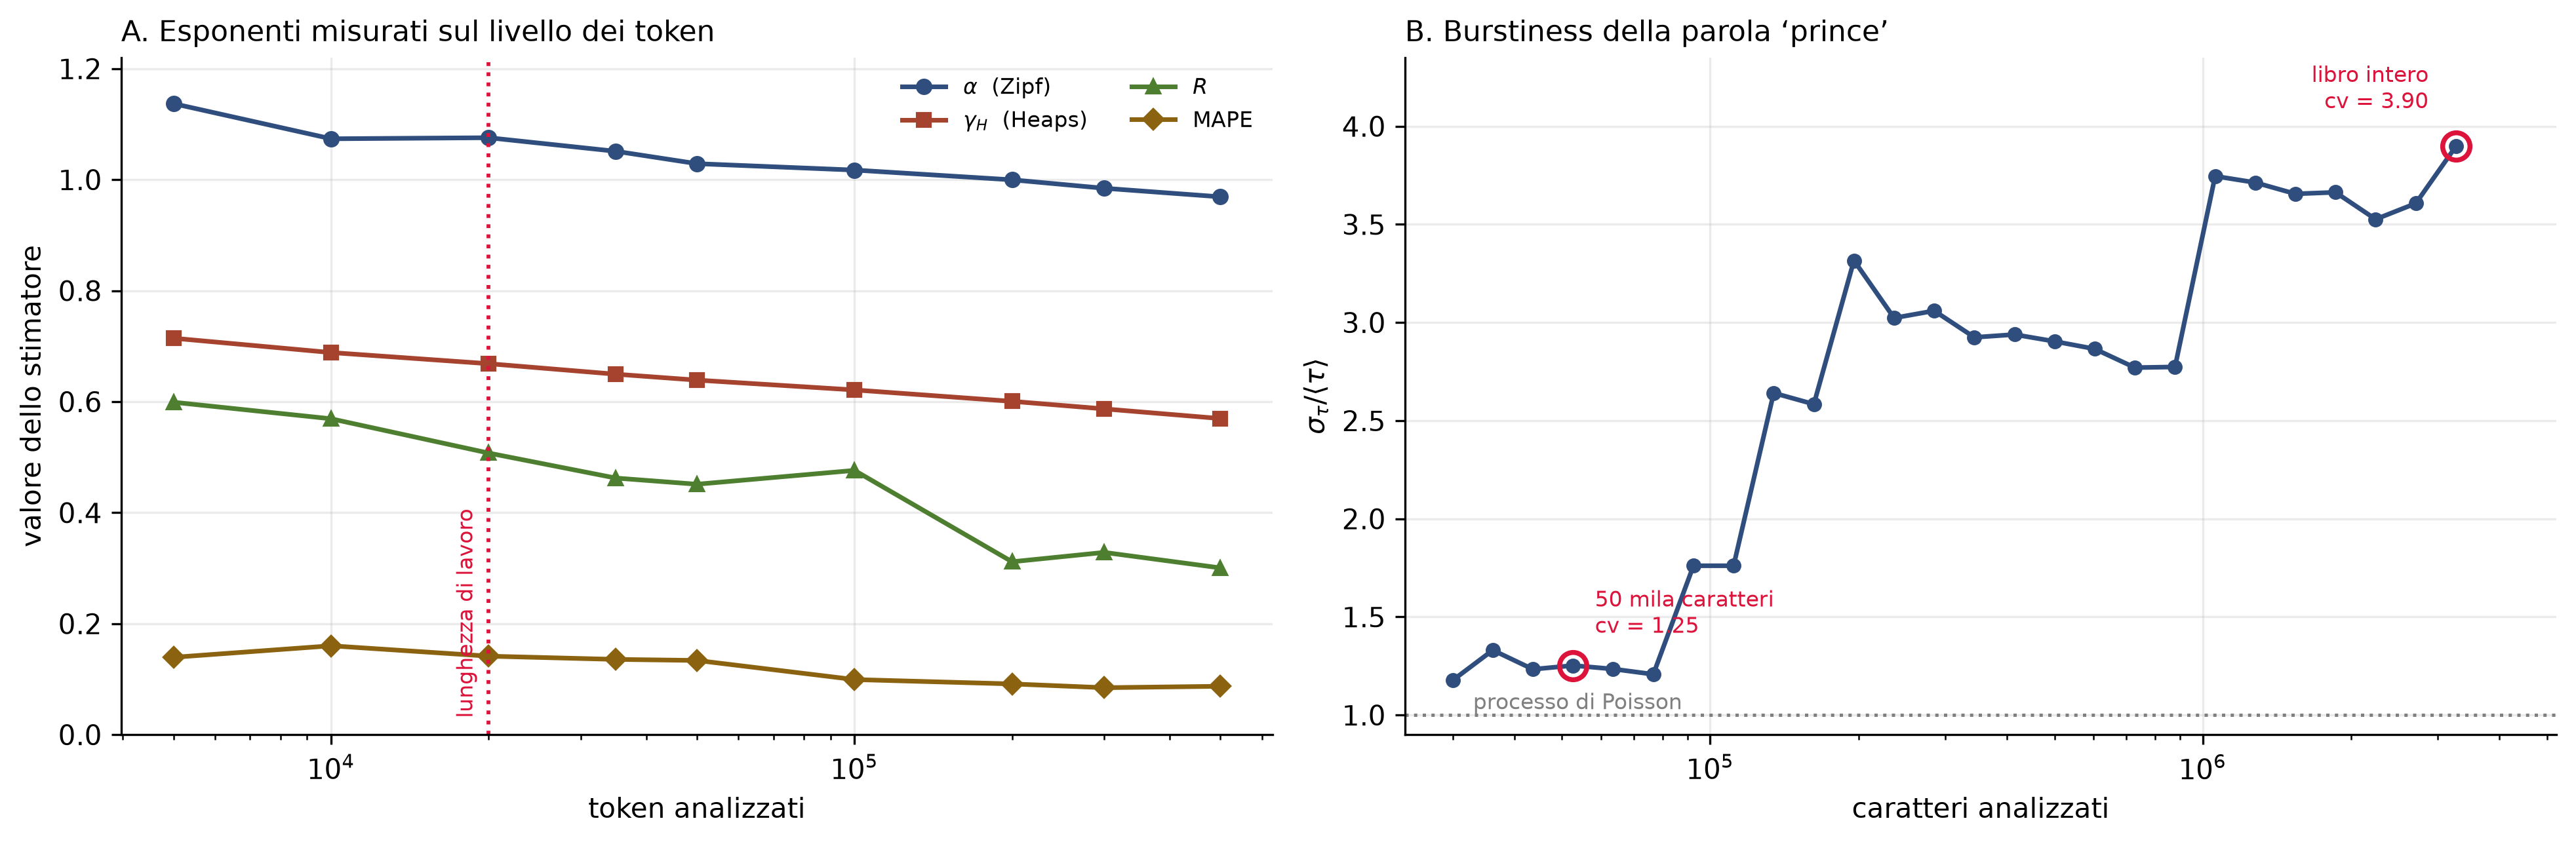
\includegraphics[width=\textwidth]{figure/cap3_dimensione_finita.png}
  \caption{Deriva degli stimatori con la lunghezza di analisi, misurata sulla
  continuazione di \emph{Guerra e pace} usata come baseline umana.
  \textbf{A}: gli esponenti misurati sul livello dei token decrescono tutti in
  modo monotono. Fra \num{5000} e \num{500000} token il descrittore $R$ passa da
  $0.60$ a $0.30$, dimezzandosi, mentre $\gamma_H$ scende da $0.72$ a $0.57$ e
  l'esponente di Zipf da $1.14$ a $0.97$. La linea verticale segna la lunghezza
  di lavoro adottata nei capitoli sperimentali.
  \textbf{B}: il coefficiente di variazione degli intervalli fra occorrenze
  della parola \emph{prince} cresce da $1.25$ su \num{50000} caratteri a $3.90$
  sul romanzo intero. La deriva è quella attesa quando la coda non
  presenta un taglio dentro la finestra osservata: finestre più lunghe
  campionano vuoti più lunghi, e la stima di $\sigma_\tau$ non raggiunge un
  valore limite. Il §\ref{sec:coda-risultati} misura direttamente il taglio e lo
  trova crescere con la finestra, da $13.5$ a $94.7$ intervalli medi fra
  \num{30000} e \num{480000} caratteri: i momenti sono finiti a ogni lunghezza,
  ma il loro valore dipende da essa.
  La Figura~\ref{fig:heaps-finito} mostrava lo stesso fenomeno su un solo
  stimatore ma su tre opere diverse, stabilendone l'universalità; qui il
  confronto è ristretto a un'unica opera e serve invece a quantificare l'entità
  dell'effetto sulla baseline effettivamente impiegata.}
  \label{fig:dimensione-finita}
\end{figure}

L'entità della deriva rende obbligatorie tre precauzioni operative, che valgono
per l'intero lavoro. Tutti i confronti fra corpora vengono condotti alla stessa
lunghezza di analisi, indicata d'ora in avanti con $N_{\mathrm{eff}}$ e
dichiarata per ciascuna fase, poiché non tutte le analisi condividono gli stessi
corpora. Nessun valore assoluto viene confrontato con valori pubblicati misurati
su lunghezze diverse. E ogni riferimento umano viene misurato con le stesse
procedure e alla stessa lunghezza dei testi con cui viene confrontato, anziché
ripreso dalla letteratura: è il paragrafo che segue. Il pannello B mostra il caso
concreto in cui la prima e la seconda precauzione si incontrano, cioè perché il
confronto con il valore pubblicato per \emph{prince} vada condotto sul romanzo
intero e non sui segmenti: è la stessa quantità, misurata su finestre che
differiscono di un fattore sessanta.

Per l'analisi appaiata dei corpora enciclopedici $N_{\mathrm{eff}}$ è fissato a
\num{60000} caratteri. Il valore è il massimo compatibile con la conservazione
di tutte le 39 terne: portandolo a \num{80000} quattro articoli non
raggiungono la soglia e le terne disponibili scendono da 39 a 35. L'intera
catena viene comunque ripetuta a quella lunghezza maggiore come controllo di
robustezza, il cui esito è riportato nel §\ref{sec:robustezza-neff} e distingue
le parti del divario che resistono al cambio di finestra da quelle che non vi
resistono.

Le altre fasi dell'analisi impiegano lunghezze diverse, perché non condividono i
corpora e non sono confrontate fra loro. La Tabella~\ref{tab:fasi} le riassume:
ciascun valore numerico che comparirà nei capitoli sperimentali è riconducibile
a una di queste righe.

\begin{table}[htbp]
\centering
\small
\begin{tabular}{@{}>{\raggedright\arraybackslash}p{2.9cm}>{\raggedright\arraybackslash}p{4.3cm}rll@{}}
\toprule
Fase & Scopo & $N_{\mathrm{eff}}$ & Unità & Analizzate \\
\midrule
Sweep di temperatura & misure sul corpus generato
  & \num{20000} & token & 242 documenti \\
\addlinespace
Raccolta & appaiamento per titolo e verifica di paternità
  & \num{80000} & caratteri & 40 coppie \\
\addlinespace
Fattibilità & verificare che l'effetto esista in prosa enciclopedica, senza
  Grokipedia & \num{50000} & caratteri & 40 voci, 20 segmenti \\
\addlinespace
Analisi principale & confronto appaiato fra i quattro corpora
  & \num{60000} & caratteri & 39 terne \\
\addlinespace
Robustezza & ripetizione dell'intera catena a lunghezza maggiore
  & \num{80000} & caratteri & 35 terne \\
\bottomrule
\end{tabular}
\caption{Le fasi dell'analisi e le rispettive lunghezze. I valori differiscono
perché le fasi non condividono i corpora, e la prima riga adotta una unità
diversa dalle altre per la ragione discussa nel §\ref{sec:unita}. Nessun
confronto attraversa righe diverse della tabella: la fase di fattibilità non
include Grokipedia, e quella sullo sweep non include alcun corpus
enciclopedico.}
\label{tab:fasi}
\end{table}

\paragraph{Baseline umana misurata, non citata.}
Per la stessa ragione, il riferimento umano non viene ripreso dalla letteratura
ma misurato con le stesse procedure e alla stessa lunghezza dei testi generati.
Il testo di riferimento è la continuazione del passaggio usato come prompt: il
confronto è quindi fra continuazione umana e continuazione generata, a parità di
contesto. La Tabella~\ref{tab:baseline} riporta i valori così ottenuti.

\begin{table}[htbp]
\centering
\small
\begin{tabular}{@{}lrr@{}}
\toprule
Grandezza & Misurata qui & Pubblicata \\
\midrule
$\alpha$ (Zipf)                 & 1.076  & $1.006 \pm 0.05$ \\
MAPE                            & 0.141  & $0.156 \pm 0.077$ \\
$\gamma_H$ (Heaps)              & 0.668  & $0.801 \pm 0.02$ \\
$R$                             & 0.507  & $0.17 \pm 0.05$ \\
$\alpha_{\mathrm{DFA}}$         & 0.579  & --- \\
$R_{\mathrm{gzip}}$             & 0.381  & --- \\
entropia [bit/carattere]        & 2.227  & --- \\
\bottomrule
\end{tabular}
\caption{Baseline umana misurata su \num{20000} token di \emph{Guerra e pace},
confrontata con i valori pubblicati in~\cite{mikhaylovskiy2025zipf}. Questi
ultimi sono calcolati su opere intere e non costituiscono un riferimento valido
per testi di questa lunghezza, per la ragione discussa nel
§\ref{sec:validazione}.}
\label{tab:baseline}
\end{table}

\paragraph{Appaiamento in frequenza dei controlli.}
Nel confronto fra parole di contenuto e parole di controllo, ciascun sostantivo
viene appaiato alla parola non-sostantivo di frequenza più vicina, minimizzando
$\lvert\log(f_w/f_k)\rvert$. L'appaiamento è indispensabile perché la burstiness
dipende dalla frequenza: confrontare parole di frequenza diversa misurerebbe
quella differenza anziché la natura semantica delle parole.

\paragraph{Selezione dei bersagli entro ciascun testo.}
Le parole bersaglio vengono scelte all'interno di ogni documento anziché fissate
una volta per tutte sul corpus di riferimento. La scelta è necessaria perché
corpora diversi trattano argomenti diversi e non condividono il lessico
tematico, ed è inoltre più efficiente, poiché produce un numero maggiore di
confronti appaiati a parità di corpus.

\paragraph{Come vengono separati i livelli lessicali.}
\label{par:livelli-lessicali}
Dentro ciascun documento le parole vengono ordinate per frequenza e ripartite in
tre insiemi. Le \emph{parole funzione} sono le sei più frequenti fra quelle che
compaiono in una lista chiusa di funtori inglesi. Le \emph{parole chiave} sono
le sette più frequenti fra quelle che superano i quattro caratteri e non
figurano in quella lista, oppure che risultano nomi propri per il criterio di
maiuscola in posizione interna alla frase descritto sopra. I \emph{controlli
appaiati} sono, per ciascuna parola chiave, la parola di frequenza più vicina
fra quelle rimaste. La ripartizione è dunque interamente determinata dalla lista
dei funtori, e la sua completezza è una scelta di metodo con conseguenze
misurabili.

La lista impiegata inizialmente conteneva \num{133} voci e ometteva alcuni
connettivi e attenuatori inglesi molto comuni, fra cui \emph{like},
\emph{amid}, \emph{including}, \emph{though}, \emph{also}, \emph{rather} e
\emph{without}. In un corpus in cui quei termini restano rari l'omissione è
innocua; in Grokipedia non lo è, perché il testo generato li impiega molto più
spesso: \emph{like} entrava fra le sette parole più frequenti in \num{29} voci
su \num{39}, contro nessuna di Wikipedia. Finivano quindi classificati come
parole chiave. Poiché i connettivi ricorrono a cadenza quasi costante e hanno
perciò burstiness bassa, il livello lessicale alto di Grokipedia risultava
contaminato da materiale che appartiene al livello dei funtori, e il divario
misurato a quel livello ne usciva gonfiato.

La lista è stata quindi estesa a \num{215} voci per classe grammaticale, cioè
preposizioni, congiunzioni subordinanti, avverbi connettivi e attenuatori e
quantificatori, e applicata identica a tutti e quattro i corpora. L'estensione
non rimuove nulla: le parole interessate passano al livello dei funtori, e al
loro posto sale fra le parole chiave la parola di contenuto successiva in
ordine di frequenza, cosicché tutti i livelli conservano la stessa numerosità
in tutti i corpora. Tutte le misure del Capitolo~\ref{cap:risultati2} sono
calcolate con la lista estesa; il §\ref{sec:effetto-stoplist} riporta di
quanto si spostano i risultati, perché lo spostamento non è trascurabile e la
scelta va resa verificabile.

% ---------------------------------------------------------------------
\section{Validazione delle procedure di calcolo}
\label{sec:validazione}

Ogni conclusione di questo lavoro poggia sul fatto che il codice misuri
effettivamente le quantità definite nel Capitolo~\ref{cap:teoria}. La
validazione procede per due vie indipendenti: la riproduzione di valori
pubblicati e la misura di grandezze il cui valore esatto è noto per costruzione.

\paragraph{Riproduzione di valori pubblicati.}
Le quantità del protocollo di Altmann sono state misurate sul corpus letterario
e confrontate con quelle riportate in~\cite{altmann2012}. Il null model A1, che
per costruzione deve restituire $\hat\gamma_{A1} \simeq 1$, dà valori compresi
fra $0.972$ e $0.984$ ai quattro livelli linguistici esaminati.

La seconda quantità riprodotta è il coefficiente di variazione della parola
\emph{prince}, che vale $3.89$ sul libro intero, in accordo con il $3.86$
pubblicato, ma scende a $1.30$ sui segmenti da \num{50000} caratteri impiegati
nei confronti. Non si tratta di un disaccordo: è la deriva di dimensione finita del
§\ref{sec:lunghezza}, e mostra perché i valori assoluti non vadano confrontati
fra lunghezze diverse. Il confronto con il valore pubblicato è quindi condotto
sul libro intero, mentre i confronti fra corpora usano la lunghezza comune.

\paragraph{Misura di esponenti noti.}
La seconda via non dipende da alcuna pubblicazione. Le procedure sono state
applicate a segnali costruiti in modo che il risultato atteso sia noto
analiticamente, ottenendo i valori della Tabella~\ref{tab:validazione}.

\begin{table}[htbp]
\centering
\small
\begin{tabular}{@{}l>{\raggedright\arraybackslash}p{5.6cm}rr@{}}
\toprule
Procedura & Segnale di prova & Atteso & Ottenuto \\
\midrule
DFA & rumore bianco & 0.500 & 0.510 \\
DFA & cammino aleatorio & 1.500 & 1.494 \\
Stimatore KL & testo confrontato con sé stesso & 0 & $0$ esatto \\
Stimatore KL & due campioni della stessa sorgente & $\simeq 0$ & 0.001 \\
Stimatore KL & sorgenti diverse & $> 0$ & 0.687 \\
\bottomrule
\end{tabular}
\caption{Validazione su segnali a esponente noto. Le prime due righe verificano
l'esponente della detrended fluctuation analysis; le ultime tre verificano che
lo stimatore della divergenza di Kullback--Leibler si annulli esattamente sul
confronto di un testo con sé stesso, resti prossimo a zero fra campioni della
stessa sorgente e cresca fra sorgenti diverse.}
\label{tab:validazione}
\end{table}

La proprietà $D(x\|x) = 0$ non è un accordo approssimato ma un'identità esatta,
e costituisce il controllo più stringente sullo stimatore della divergenza:
come discusso nel §\ref{sec:crossparsing}, essa vale soltanto se i riferimenti
usati nei due termini hanno la stessa lunghezza, e una sua violazione
segnalerebbe immediatamente l'errore.

% ---------------------------------------------------------------------
\section{Controlli di robustezza}
\label{sec:robustezza}

I controlli di questa sezione non verificano che le procedure siano corrette, ma
che i risultati non dipendano da scelte che avrebbero potuto essere compiute
diversamente.

\paragraph{Ordine del detrending.}
La detrended fluctuation analysis rimuove dalle finestre le tendenze polinomiali
fino a un grado fissato. L'intera analisi è stata condotta con il grado 1 e con
il grado 2, e la Tabella~\ref{tab:ordine-dfa} riporta le due stime a ciascuna
temperatura. Le misure riportate nel Capitolo~\ref{cap:risultati1} usano il
grado 2, per la ragione che il confronto stesso rende evidente: dove il segnale
è stazionario i due gradi coincidono, e dove non lo è il grado 1 restituisce un
esponente sistematicamente più alto, perché lascia nel segnale una tendenza che
non è correlazione.

\begin{table}[htbp]
\centering
\small
\begin{tabular}{@{}lrrrrr@{}}
\toprule
$T$ & grado 1 & grado 2 & scarto & dispersione & documenti \\
\midrule
0.4 & 0.284 & 0.307 & $-0.046$ & 0.085 & 21 \\
0.5 & 0.582 & 0.500 & $-0.132$ & 0.081 & 21 \\
0.6 & 0.613 & 0.416 & $-0.124$ & 0.093 & 21 \\
0.7 & 0.713 & 0.583 & $-0.115$ & 0.073 & 21 \\
0.8 & 0.715 & 0.601 & $-0.138$ & 0.070 & 20 \\
0.9 & 0.758 & 0.659 & $-0.078$ & 0.050 & 18 \\
1.0 & 0.753 & 0.711 & $-0.014$ & 0.054 & 17 \\
1.1 & 0.651 & 0.564 & $-0.060$ & 0.046 & 19 \\
1.2 & 0.570 & 0.556 & $-0.029$ & 0.035 & 21 \\
1.3 & 0.563 & 0.535 & $-0.007$ & 0.024 & 21 \\
1.4 & 0.535 & 0.532 & $-0.009$ & 0.019 & 21 \\
1.5 & 0.529 & 0.527 & $-0.006$ & 0.015 & 21 \\
\midrule
\multicolumn{3}{@{}l}{testo umano} & $-0.007$ & --- & 1 \\
\bottomrule
\end{tabular}
\caption{Esponente della fluttuazione stimato con detrending di grado 1 e di
grado 2. Le prime tre colonne numeriche riportano mediane sui documenti
disponibili a ciascuna temperatura; la quarta è la deviazione standard dello
scarto fra i due gradi, calcolata documento per documento. Lo scarto è negativo
ovunque, come atteso, perché il grado 2 rimuove tendenze che il grado 1 lascia
nel segnale.}
\label{tab:ordine-dfa}
\end{table}

Le due stime coincidono dove il segnale è stazionario. Sulla baseline umana lo
scarto vale $-0.007$, e sui testi generati da $T = 1.2$ in su la sua mediana vale
$-0.010$ a fronte di una dispersione fra documenti di $0.027$: la differenza fra
i due gradi è più piccola della variabilità fra documenti generati nelle stesse
condizioni, e l'esponente non dipende in modo apprezzabile dalla scelta del
detrending.

Nell'intervallo $T \in [0.5, 0.8]$ lo scarto mediano vale invece $-0.125$, con
dispersione $0.078$: qui la differenza supera nettamente la variabilità ed è
quindi reale. È concentrata nel regime in cui il testo degenera in cicli di
ripetizione e la serie dei ranghi non è stazionaria, e in quel regime,
coerentemente con quanto osservato nel §\ref{sec:ponte}, l'esponente va letto
come indicatore di periodicità e non come misura di correlazione a lungo raggio.


\paragraph{Numerosità disuguale fra celle.}
Dalla disuguale numerosità dichiarata nel §\ref{sec:protocollo} discendono due
limitazioni. Per il modello da 14 miliardi di parametri non esiste una stima
della dispersione fra campioni, cosicché nelle sue figure le barre d'errore non
sono definite e ogni suo valore è una singola realizzazione; e le deviazioni
standard riportate nelle figure del Capitolo~\ref{cap:risultati1} non sono
confrontabili fra modelli, poiché derivano da un numero diverso di campioni. Le
conclusioni che riguardano il confronto fra modelli vanno lette con questa
avvertenza, che il §\ref{sec:zipf-risultati} riprende quantitativamente sul
caso in cui pesa di più.

% ---------------------------------------------------------------------
\section{Riproducibilità}
\label{sec:riproducibilita}

Tutte le procedure sono deterministiche a semi fissati, e i semi impiegati sono
registrati nel codice. I corpora scaricati da fonti esterne sono conservati in
copia locale, così che una modifica successiva della fonte non alteri i
risultati: vale in particolare per le voci di Grokipedia, che vengono riscritte
senza cronologia pubblica.

I dati intermedi e le figure sono prodotti da notebook che salvano ogni risultato
in file separati, in formato aperto, insieme a una sintesi testuale dei
parametri usati e delle scelte compiute, così che ciascuna figura sia
ricostruibile senza ripetere i calcoli.

% =====================================================================

\chapter{Materiali e metodi}
\label{cap:metodi}

Questo capitolo descrive i corpora analizzati, il protocollo con cui i testi
artificiali sono stati prodotti e le scelte metodologiche comuni alle due parti
sperimentali. Il criterio seguito nell'esposizione è che un lettore debba poter
ripetere l'intera analisi senza dover chiedere nulla: ogni scelta viene perciò
motivata e non soltanto dichiarata.

Le ultime tre sezioni sono dedicate ai controlli. Il §\ref{sec:validazione}
verifica che le procedure di calcolo misurino effettivamente le quantità
definite nel Capitolo~\ref{cap:teoria}; il §\ref{sec:robustezza} verifica che i
risultati non dipendano da scelte arbitrarie. Sono due questioni distinte, e
tenerle separate rende più chiaro che cosa ciascun controllo dimostri.

% ---------------------------------------------------------------------
\section{I corpora}
\label{sec:corpora}

L'analisi impiega cinque corpora, riassunti nella Tabella~\ref{tab:corpora}.
Due sono di riferimento umano, due sono enciclopedie messe a confronto fra loro,
e uno raccoglie i testi generati automaticamente.

\begin{table}[htbp]
\centering
\small
\begin{tabular}{@{}l>{\raggedright\arraybackslash}p{5.9cm}c@{}}
\toprule
Corpus & Provenienza e criterio di selezione & Unità \\
\midrule
\emph{Guerra e pace} & Project Gutenberg; segmenti contigui di uguale lunghezza,
usati come ancora al protocollo originale & 20 segmenti \\
\addlinespace
Wikipedia & voci a tema ampio, selezionate ordinando per lunghezza di prosa
effettiva & 40 raccolte, 39 analizzate \\
\addlinespace
Grokipedia (attuale) & le stesse voci, appaiate per titolo & 40 raccolte, 39
analizzate \\
\addlinespace
Grokipedia v0.1 & le stesse voci nella versione di ottobre 2025, recuperata da
Internet Archive & 40 raccolte, 39 analizzate \\
\addlinespace
Testi generati & cinque modelli Qwen, sweep di temperatura descritto nel
§\ref{sec:protocollo} & 242 documenti \\
\bottomrule
\end{tabular}
\caption{I corpora analizzati.}
\label{tab:corpora}
\end{table}

Il corpus letterario ha una funzione precisa: fornire un'ancora al protocollo di
Altmann~\cite{altmann2012}, che è stato formulato e validato su romanzi. I valori
misurati su di esso permettono di verificare che la procedura riproduca quanto
pubblicato prima di applicarla a testi di natura diversa.

Le voci di Wikipedia sono state ordinate per lunghezza del solo testo corrente,
dopo rimozione di marcatura, tabelle, note e riferimenti. I due criteri più
immediati non sono utilizzabili. Ordinare le pagine per dimensione del sorgente
wiki restituisce liste, tabelle e infobox anziché prosa: una pagina da
\num{679016} byte di sorgente conteneva \num{1284} caratteri di prosa effettiva.
Ordinare per qualità editoriale è ugualmente inadatto, poiché le voci in vetrina
sono selezionate per accuratezza e non per lunghezza.

Grokipedia compare in due versioni perché la piattaforma non pubblica una
cronologia delle revisioni. La versione di ottobre 2025 è stata recuperata da
Internet Archive, disponibile per tutte e quaranta le voci, e consente di
verificare se gli indicatori misurati cambino a seguito della revisione
editoriale: è il controllo riportato nel Capitolo~\ref{cap:risultati2}.

% ---------------------------------------------------------------------
\section{Protocollo di generazione}
\label{sec:protocollo}

I testi artificiali sono stati prodotti da cinque modelli della famiglia Qwen,
elencati nella Tabella~\ref{tab:modelli}. Tutti sono modelli \emph{base}, cioè
non sottoposti ad affinamento su istruzioni: la scelta isola le proprietà del
modello linguistico da quelle indotte dall'addestramento successivo, che
in~\cite{mikhaylovskiy2025zipf} risultano spostare sensibilmente il
comportamento statistico.

\begin{table}[htbp]
\centering
\small
\begin{tabular}{@{}llrlr@{}}
\toprule
Modello & Famiglia & Parametri & Architettura & Documenti \\
\midrule
Qwen2.5-1.5B     & Qwen2.5 & 1.54\,G  & transformer denso & 57 \\
Qwen2.5-3B       & Qwen2.5 & 3.09\,G  & transformer denso & 53 \\
Qwen2.5-14B      & Qwen2.5 & 14.7\,G  & transformer denso & 12 \\
Qwen3.5-2B-Base  & Qwen3.5 & 2.0\,G   & ibrida            & 60 \\
Qwen3.5-4B-Base  & Qwen3.5 & 4.0\,G   & ibrida            & 60 \\
\midrule
\multicolumn{4}{@{}l}{totale} & 242 \\
\bottomrule
\end{tabular}
\caption{I cinque modelli impiegati. L'intervallo di dimensioni copre un ordine
di grandezza, e le due famiglie differiscono per architettura. I modelli
Qwen2.5 sono transformer densi ad attenzione completa su tutti gli strati; i
modelli Qwen3.5 sono ibridi e ripetono un blocco di quattro strati in cui tre
impiegano attenzione lineare e uno attenzione completa. Le schede ufficiali
riportano \num{24} strati per il modello da 2 miliardi di parametri, come
$6\times(3\times\text{lineare} + 1\times\text{completa})$, e \num{32} per
quello da 4 miliardi, come $8\times(3+1)$: in entrambi i casi tre quarti degli
strati sono ad attenzione lineare.}
\label{tab:modelli}
\end{table}

Ogni modello ha generato testo a dodici temperature, da $T = 0.4$ a $T = 1.5$
con passo $0.1$. Il prompt è identico per tutti: un blocco di 2000 token tratto
da \emph{Guerra e pace}, la cui posizione esatta nel romanzo è stata verificata
come descritto nel §\ref{sec:paternita}. Ciascuna generazione produce
\num{24000} token di completamento, misurati con il tokenizzatore del modello
generante.

\paragraph{Che cosa comporta un prompt lungo.}
La scelta di un prompt di 2000 token non è neutra rispetto alle misure, e la
conseguenza è anticipata qui perché ricorre in tutto il
Capitolo~\ref{cap:risultati1}. La sezione 4.5
di~\cite{mikhaylovskiy2025zipf} ripete lo sweep con un prompt di quella
lunghezza tratto da un testo naturale e osserva che la ricchezza lessicale del
prompt domina il vocabolario, relativamente piccolo, del testo generato: alcuni
modelli non producono alcun tipo nuovo alle basse temperature, i massimi delle
curve del descrittore $R$ si spostano verso le temperature alte, e l'errore del
fit di Zipf si abbassa soprattutto nella regione a bassa temperatura. Le
proprietà del regime disordinato compaiono dunque più tardi, e quelle del
regime ordinato persistono più a lungo, di quanto si osserverebbe generando da
un singolo token. I confronti con i valori pubblicati vanno letti tenendone
conto, e i punti in cui l'effetto si manifesta sono segnalati di volta in
volta.

Il campionamento impiega la sola temperatura. I parametri che troncano la
distribuzione sono disattivati, con $\mathrm{top}\text{-}p = 1$ e
$\mathrm{top}\text{-}k = -1$, e la penalità di ripetizione è posta a 1. È la
condizione richiesta dal §\ref{sec:temperatura}: qualunque altro parametro
introdurrebbe un secondo grado di libertà e renderebbe impossibile attribuire
alla sola temperatura il comportamento osservato.

\paragraph{Generazione in continuazione.}
Per raggiungere i \num{24000} token richiesti la generazione riparte dopo ogni
token di fine sequenza, riprendendo dal testo accumulato fino a quel punto. I
documenti prodotti sono dunque ricuciti da più segmenti, in numero variabile fino
a un massimo di 27 riprese per campione. Poiché un modello autoregressivo è privo
di stato interno persistente, riprendere dal testo accumulato produce la stessa
distribuzione condizionata. Un confronto a temperatura fissata fra i documenti
ricuciti da più segmenti e quelli generati in un colpo solo non rivela
differenze nelle due misure sensibili all'ordine, entro la dispersione dei dati;
il confronto ha però poca potenza, perché sotto $T = 0.9$ i documenti con
riprese sono pochissimi e sopra $T = 1.0$ la ripetizione è già nulla.

\paragraph{Numerosità disuguale.}
Il numero di documenti per modello non è uniforme, e la
Tabella~\ref{tab:modelli} lo riporta esplicitamente: il modello da 14 miliardi
di parametri dispone di un solo campione per temperatura, contro i cinque della
maggior parte degli altri. Le conseguenze sono discusse fra i limiti nel
§\ref{sec:robustezza}.

% ---------------------------------------------------------------------
\section{Verifica di paternità dei corpora}
\label{sec:paternita}

Il confronto fra Wikipedia e Grokipedia presuppone che le voci della seconda
siano effettivamente scritte da un modello generativo e non ricopiate dalla
prima. La verifica misura la sovrapposizione di 8-grammi fra le due versioni di
ciascuna voce: sul corpus attuale la mediana vale $0.0003$ e il massimo $0.046$,
valori che escludono la derivazione testuale diretta. Una voce della versione
v0.1, \emph{Buddhism}, risultava invece ricopiata all'84\% ed è stata esclusa
dall'analisi appaiata, che si riduce quindi a 39 terne: il disegno richiede
infatti che tutte e tre le versioni siano disponibili per ogni titolo, per cui
l'esclusione di una versione comporta quella dell'intera terna.

Per i testi generati la verifica riguarda il prompt. Poiché i cinque dataset sono
stati prodotti in momenti diversi, occorre accertare che partano tutti dallo
stesso punto del romanzo. Il controllo non è stato condotto per ispezione ma per
funzione di hash: dell'impronta SHA-256 registrata in ciascun dataset è stata
cercata la corrispondenza nel testo del romanzo, individuando l'offset esatto in
caratteri. Tutti e cinque i dataset risultano partire dalla stessa posizione. Due
di essi registrano una lunghezza del prompt di poco diversa, \num{8239} contro
\num{8262} caratteri, differenza dovuta al punto in cui cade il confine dei 2000
token con i due tokenizzatori delle rispettive famiglie e non a un testo diverso.

% ---------------------------------------------------------------------
\section{Unità di analisi}
\label{sec:unita}

La scelta dell'unità in cui misurare i testi è la decisione metodologica di
maggiore conseguenza dell'intero lavoro, e viene qui motivata per esteso.

Il livello primario è il token, non la parola. La ragione, già anticipata nel
§\ref{sec:token}, è che alle temperature alte i modelli producono sequenze non
interpretabili come parole: una tokenizzazione lessicale misurerebbe in quel
regime artefatti della segmentazione anziché proprietà del testo. La stessa
scelta, e per lo stesso motivo, è compiuta in~\cite{mikhaylovskiy2025zipf}.

Il tokenizzatore impiegato nell'analisi è unico per tutti i corpora ed è esterno
alle famiglie che hanno generato i testi. Le due condizioni sono entrambe
necessarie. L'unicità serve a rendere confrontabili gli esponenti misurati su
modelli diversi: i tokenizzatori di Qwen2.5 e Qwen3.5 segmentano lo stesso testo
in modo diverso, e misurare ciascun modello con il proprio metro produrrebbe
differenze attribuibili alla segmentazione anziché al testo. L'esternalità serve
a evitare che un modello risulti favorito dal fatto di essere misurato con il
proprio vocabolario. La scelta ricalca quella di~\cite{mikhaylovskiy2025zipf},
dove testi prodotti da quattro famiglie distinte vengono analizzati con un
tokenizzatore che non appartiene a nessuna di esse.

In concreto l'analisi impiega \texttt{cl100k\_base}, con \num{100277} voci.
Cambiare tokenizzatore sposta i valori assoluti degli esponenti, poiché cambia
l'unità in cui si contano le occorrenze, ma non la posizione dei loro estremi in
funzione della temperatura, che è la quantità su cui poggiano le conclusioni del
Capitolo~\ref{cap:risultati1}.

Ogni documento generato viene troncato ai primi \num{20000} token di analisi, e
la baseline umana è misurata sulla stessa quantità. Il valore è il massimo
compatibile con il documento più corto del corpus: la generazione produce
\num{24000} token misurati con il tokenizzatore del modello generante, che
\texttt{cl100k\_base} risegmenta in un numero variabile di token di analisi, e
troncare a una soglia comune è indispensabile perché tutte le misure del
Capitolo~\ref{cap:risultati1} dipendono dalla lunghezza. La prima riga della
Tabella~\ref{tab:fasi} riporta questa fase; le altre adottano il carattere come
unità, perché il protocollo del §\ref{sec:burst} misura le distanze in
caratteri.

Il livello lessicale resta impiegato, in funzione secondaria, per le misure che
sono definite sulle parole: la diversità lessicale, le distanze di ripetizione,
gli $n$-grammi ripetuti e la mappatura sui vettori di embedding. La detrended
fluctuation analysis fa eccezione a entrambi i livelli, poiché
in~\cite{lippi2019} è definita sui caratteri, e qui si segue quella definizione.

% ---------------------------------------------------------------------
\section{Scelte metodologiche trasversali}
\label{sec:scelte}

Quattro decisioni attraversano entrambe le parti sperimentali.

\paragraph{Lunghezza di analisi comune.}
Come anticipato nel §\ref{sec:lunghezza}, diversi stimatori impiegati in questo
lavoro non convergono al crescere della lunghezza del testo, ma derivano in modo
sistematico. La Figura~\ref{fig:dimensione-finita} misura la deriva su un testo
umano, e mostra che non si tratta di un effetto trascurabile.

\begin{figure}[htbp]
  \centering
  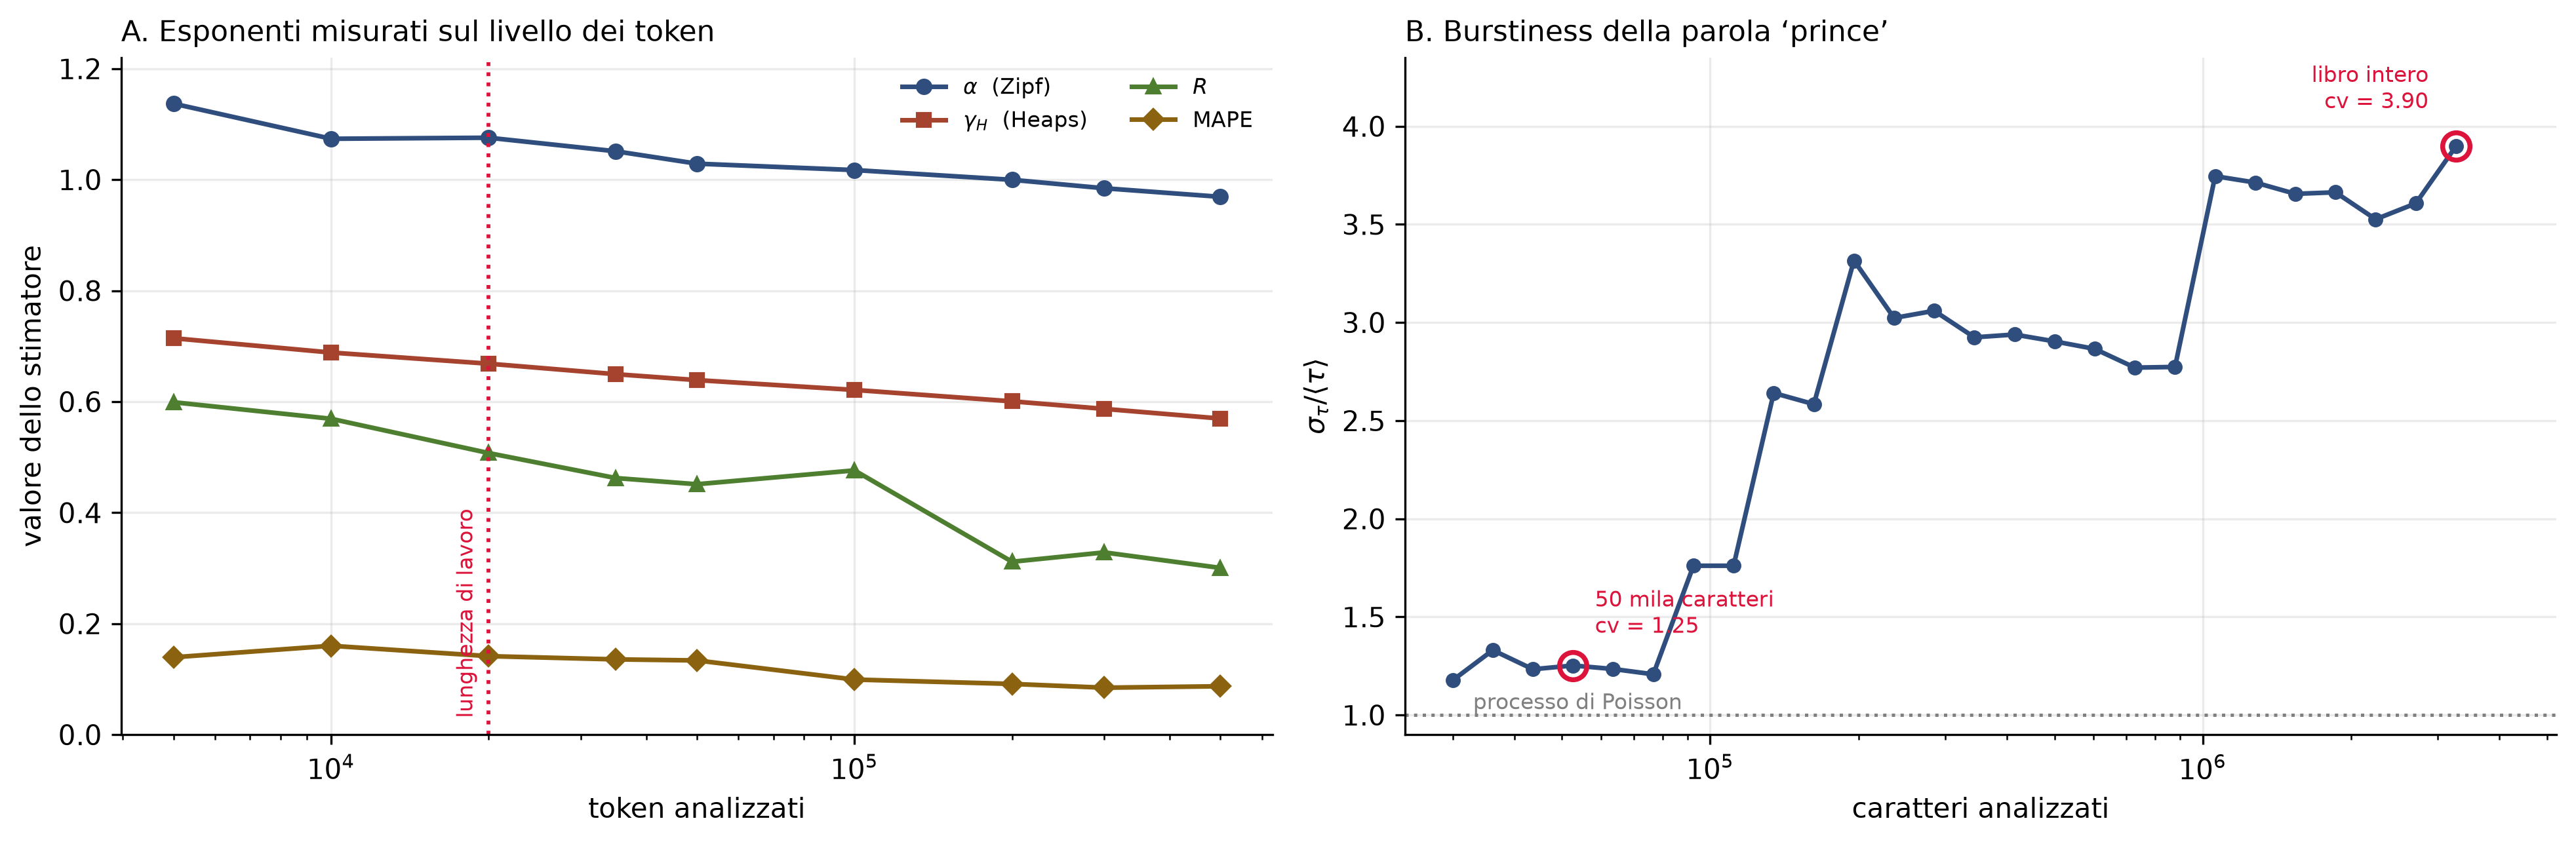
\includegraphics[width=\textwidth]{figure/cap3_dimensione_finita.png}
  \caption{Deriva degli stimatori con la lunghezza di analisi, misurata sulla
  continuazione di \emph{Guerra e pace} usata come baseline umana.
  \textbf{A}: gli esponenti misurati sul livello dei token decrescono tutti in
  modo monotono. Fra \num{5000} e \num{500000} token il descrittore $R$ passa da
  $0.60$ a $0.30$, dimezzandosi, mentre $\gamma_H$ scende da $0.72$ a $0.57$ e
  l'esponente di Zipf da $1.14$ a $0.97$. La linea verticale segna la lunghezza
  di lavoro adottata nei capitoli sperimentali.
  \textbf{B}: il coefficiente di variazione degli intervalli fra occorrenze
  della parola \emph{prince} cresce da $1.25$ su \num{50000} caratteri a $3.90$
  sul romanzo intero. La deriva è quella attesa quando la coda non
  presenta un taglio dentro la finestra osservata: finestre più lunghe
  campionano vuoti più lunghi, e la stima di $\sigma_\tau$ non raggiunge un
  valore limite. Il §\ref{sec:coda-risultati} misura direttamente il taglio e lo
  trova crescere con la finestra, da $13.5$ a $94.7$ intervalli medi fra
  \num{30000} e \num{480000} caratteri: i momenti sono finiti a ogni lunghezza,
  ma il loro valore dipende da essa.
  La Figura~\ref{fig:heaps-finito} mostrava lo stesso fenomeno su un solo
  stimatore ma su tre opere diverse, stabilendone l'universalità; qui il
  confronto è ristretto a un'unica opera e serve invece a quantificare l'entità
  dell'effetto sulla baseline effettivamente impiegata.}
  \label{fig:dimensione-finita}
\end{figure}

L'entità della deriva rende obbligatorie tre precauzioni operative, che valgono
per l'intero lavoro. Tutti i confronti fra corpora vengono condotti alla stessa
lunghezza di analisi, indicata d'ora in avanti con $N_{\mathrm{eff}}$ e
dichiarata per ciascuna fase, poiché non tutte le analisi condividono gli stessi
corpora. Nessun valore assoluto viene confrontato con valori pubblicati misurati
su lunghezze diverse. E ogni riferimento umano viene misurato con le stesse
procedure e alla stessa lunghezza dei testi con cui viene confrontato, anziché
ripreso dalla letteratura: è il paragrafo che segue. Il pannello B mostra il caso
concreto in cui la prima e la seconda precauzione si incontrano, cioè perché il
confronto con il valore pubblicato per \emph{prince} vada condotto sul romanzo
intero e non sui segmenti: è la stessa quantità, misurata su finestre che
differiscono di un fattore sessanta.

Per l'analisi appaiata dei corpora enciclopedici $N_{\mathrm{eff}}$ è fissato a
\num{60000} caratteri. Il valore è il massimo compatibile con la conservazione
di tutte le 39 terne: portandolo a \num{80000} quattro articoli non
raggiungono la soglia e le terne disponibili scendono da 39 a 35. L'intera
catena viene comunque ripetuta a quella lunghezza maggiore come controllo di
robustezza, il cui esito è riportato nel §\ref{sec:robustezza-neff} e distingue
le parti del divario che resistono al cambio di finestra da quelle che non vi
resistono.

Le altre fasi dell'analisi impiegano lunghezze diverse, perché non condividono i
corpora e non sono confrontate fra loro. La Tabella~\ref{tab:fasi} le riassume:
ciascun valore numerico che comparirà nei capitoli sperimentali è riconducibile
a una di queste righe.

\begin{table}[htbp]
\centering
\small
\begin{tabular}{@{}>{\raggedright\arraybackslash}p{2.9cm}>{\raggedright\arraybackslash}p{4.3cm}rll@{}}
\toprule
Fase & Scopo & $N_{\mathrm{eff}}$ & Unità & Analizzate \\
\midrule
Sweep di temperatura & misure sul corpus generato
  & \num{20000} & token & 242 documenti \\
\addlinespace
Raccolta & appaiamento per titolo e verifica di paternità
  & \num{80000} & caratteri & 40 coppie \\
\addlinespace
Fattibilità & verificare che l'effetto esista in prosa enciclopedica, senza
  Grokipedia & \num{50000} & caratteri & 40 voci, 20 segmenti \\
\addlinespace
Analisi principale & confronto appaiato fra i quattro corpora
  & \num{60000} & caratteri & 39 terne \\
\addlinespace
Robustezza & ripetizione dell'intera catena a lunghezza maggiore
  & \num{80000} & caratteri & 35 terne \\
\bottomrule
\end{tabular}
\caption{Le fasi dell'analisi e le rispettive lunghezze. I valori differiscono
perché le fasi non condividono i corpora, e la prima riga adotta una unità
diversa dalle altre per la ragione discussa nel §\ref{sec:unita}. Nessun
confronto attraversa righe diverse della tabella: la fase di fattibilità non
include Grokipedia, e quella sullo sweep non include alcun corpus
enciclopedico.}
\label{tab:fasi}
\end{table}

\paragraph{Baseline umana misurata, non citata.}
Per la stessa ragione, il riferimento umano non viene ripreso dalla letteratura
ma misurato con le stesse procedure e alla stessa lunghezza dei testi generati.
Il testo di riferimento è la continuazione del passaggio usato come prompt: il
confronto è quindi fra continuazione umana e continuazione generata, a parità di
contesto. La Tabella~\ref{tab:baseline} riporta i valori così ottenuti.

\begin{table}[htbp]
\centering
\small
\begin{tabular}{@{}lrr@{}}
\toprule
Grandezza & Misurata qui & Pubblicata \\
\midrule
$\alpha$ (Zipf)                 & 1.076  & $1.006 \pm 0.05$ \\
MAPE                            & 0.141  & $0.156 \pm 0.077$ \\
$\gamma_H$ (Heaps)              & 0.668  & $0.801 \pm 0.02$ \\
$R$                             & 0.507  & $0.17 \pm 0.05$ \\
$\alpha_{\mathrm{DFA}}$         & 0.579  & --- \\
$R_{\mathrm{gzip}}$             & 0.381  & --- \\
entropia [bit/carattere]        & 2.227  & --- \\
\bottomrule
\end{tabular}
\caption{Baseline umana misurata su \num{20000} token di \emph{Guerra e pace},
confrontata con i valori pubblicati in~\cite{mikhaylovskiy2025zipf}. Questi
ultimi sono calcolati su opere intere e non costituiscono un riferimento valido
per testi di questa lunghezza, per la ragione discussa nel
§\ref{sec:validazione}.}
\label{tab:baseline}
\end{table}

\paragraph{Appaiamento in frequenza dei controlli.}
Nel confronto fra parole di contenuto e parole di controllo, ciascun sostantivo
viene appaiato alla parola non-sostantivo di frequenza più vicina, minimizzando
$\lvert\log(f_w/f_k)\rvert$. L'appaiamento è indispensabile perché la burstiness
dipende dalla frequenza: confrontare parole di frequenza diversa misurerebbe
quella differenza anziché la natura semantica delle parole.

\paragraph{Selezione dei bersagli entro ciascun testo.}
Le parole bersaglio vengono scelte all'interno di ogni documento anziché fissate
una volta per tutte sul corpus di riferimento. La scelta è necessaria perché
corpora diversi trattano argomenti diversi e non condividono il lessico
tematico, ed è inoltre più efficiente, poiché produce un numero maggiore di
confronti appaiati a parità di corpus.

\paragraph{Come vengono separati i livelli lessicali.}
\label{par:livelli-lessicali}
Dentro ciascun documento le parole vengono ordinate per frequenza e ripartite in
tre insiemi. Le \emph{parole funzione} sono le sei più frequenti fra quelle che
compaiono in una lista chiusa di funtori inglesi. Le \emph{parole chiave} sono
le sette più frequenti fra quelle che superano i quattro caratteri e non
figurano in quella lista, oppure che risultano nomi propri per il criterio di
maiuscola in posizione interna alla frase descritto sopra. I \emph{controlli
appaiati} sono, per ciascuna parola chiave, la parola di frequenza più vicina
fra quelle rimaste. La ripartizione è dunque interamente determinata dalla lista
dei funtori, e la sua completezza è una scelta di metodo con conseguenze
misurabili.

La lista impiegata inizialmente conteneva \num{133} voci e ometteva alcuni
connettivi e attenuatori inglesi molto comuni, fra cui \emph{like},
\emph{amid}, \emph{including}, \emph{though}, \emph{also}, \emph{rather} e
\emph{without}. In un corpus in cui quei termini restano rari l'omissione è
innocua; in Grokipedia non lo è, perché il testo generato li impiega molto più
spesso: \emph{like} entrava fra le sette parole più frequenti in \num{29} voci
su \num{39}, contro nessuna di Wikipedia. Finivano quindi classificati come
parole chiave. Poiché i connettivi ricorrono a cadenza quasi costante e hanno
perciò burstiness bassa, il livello lessicale alto di Grokipedia risultava
contaminato da materiale che appartiene al livello dei funtori, e il divario
misurato a quel livello ne usciva gonfiato.

La lista è stata quindi estesa a \num{215} voci per classe grammaticale, cioè
preposizioni, congiunzioni subordinanti, avverbi connettivi e attenuatori e
quantificatori, e applicata identica a tutti e quattro i corpora. L'estensione
non rimuove nulla: le parole interessate passano al livello dei funtori, e al
loro posto sale fra le parole chiave la parola di contenuto successiva in
ordine di frequenza, cosicché tutti i livelli conservano la stessa numerosità
in tutti i corpora. Tutte le misure del Capitolo~\ref{cap:risultati2} sono
calcolate con la lista estesa; il §\ref{sec:effetto-stoplist} riporta di
quanto si spostano i risultati, perché lo spostamento non è trascurabile e la
scelta va resa verificabile.

% ---------------------------------------------------------------------
\section{Validazione delle procedure di calcolo}
\label{sec:validazione}

Ogni conclusione di questo lavoro poggia sul fatto che il codice misuri
effettivamente le quantità definite nel Capitolo~\ref{cap:teoria}. La
validazione procede per due vie indipendenti: la riproduzione di valori
pubblicati e la misura di grandezze il cui valore esatto è noto per costruzione.

\paragraph{Riproduzione di valori pubblicati.}
Le quantità del protocollo di Altmann sono state misurate sul corpus letterario
e confrontate con quelle riportate in~\cite{altmann2012}. Il null model A1, che
per costruzione deve restituire $\hat\gamma_{A1} \simeq 1$, dà valori compresi
fra $0.972$ e $0.984$ ai quattro livelli linguistici esaminati.

La seconda quantità riprodotta è il coefficiente di variazione della parola
\emph{prince}, che vale $3.89$ sul libro intero, in accordo con il $3.86$
pubblicato, ma scende a $1.30$ sui segmenti da \num{50000} caratteri impiegati
nei confronti. Non si tratta di un disaccordo: è la deriva di dimensione finita del
§\ref{sec:lunghezza}, e mostra perché i valori assoluti non vadano confrontati
fra lunghezze diverse. Il confronto con il valore pubblicato è quindi condotto
sul libro intero, mentre i confronti fra corpora usano la lunghezza comune.

\paragraph{Misura di esponenti noti.}
La seconda via non dipende da alcuna pubblicazione. Le procedure sono state
applicate a segnali costruiti in modo che il risultato atteso sia noto
analiticamente, ottenendo i valori della Tabella~\ref{tab:validazione}.

\begin{table}[htbp]
\centering
\small
\begin{tabular}{@{}l>{\raggedright\arraybackslash}p{5.6cm}rr@{}}
\toprule
Procedura & Segnale di prova & Atteso & Ottenuto \\
\midrule
DFA & rumore bianco & 0.500 & 0.510 \\
DFA & cammino aleatorio & 1.500 & 1.494 \\
Stimatore KL & testo confrontato con sé stesso & 0 & $0$ esatto \\
Stimatore KL & due campioni della stessa sorgente & $\simeq 0$ & 0.001 \\
Stimatore KL & sorgenti diverse & $> 0$ & 0.687 \\
\bottomrule
\end{tabular}
\caption{Validazione su segnali a esponente noto. Le prime due righe verificano
l'esponente della detrended fluctuation analysis; le ultime tre verificano che
lo stimatore della divergenza di Kullback--Leibler si annulli esattamente sul
confronto di un testo con sé stesso, resti prossimo a zero fra campioni della
stessa sorgente e cresca fra sorgenti diverse.}
\label{tab:validazione}
\end{table}

La proprietà $D(x\|x) = 0$ non è un accordo approssimato ma un'identità esatta,
e costituisce il controllo più stringente sullo stimatore della divergenza:
come discusso nel §\ref{sec:crossparsing}, essa vale soltanto se i riferimenti
usati nei due termini hanno la stessa lunghezza, e una sua violazione
segnalerebbe immediatamente l'errore.

% ---------------------------------------------------------------------
\section{Controlli di robustezza}
\label{sec:robustezza}

I controlli di questa sezione non verificano che le procedure siano corrette, ma
che i risultati non dipendano da scelte che avrebbero potuto essere compiute
diversamente.

\paragraph{Ordine del detrending.}
La detrended fluctuation analysis rimuove dalle finestre le tendenze polinomiali
fino a un grado fissato. L'intera analisi è stata condotta con il grado 1 e con
il grado 2, e la Tabella~\ref{tab:ordine-dfa} riporta le due stime a ciascuna
temperatura. Le misure riportate nel Capitolo~\ref{cap:risultati1} usano il
grado 2, per la ragione che il confronto stesso rende evidente: dove il segnale
è stazionario i due gradi coincidono, e dove non lo è il grado 1 restituisce un
esponente sistematicamente più alto, perché lascia nel segnale una tendenza che
non è correlazione.

\begin{table}[htbp]
\centering
\small
\begin{tabular}{@{}lrrrrr@{}}
\toprule
$T$ & grado 1 & grado 2 & scarto & dispersione & documenti \\
\midrule
0.4 & 0.284 & 0.307 & $-0.046$ & 0.085 & 21 \\
0.5 & 0.582 & 0.500 & $-0.132$ & 0.081 & 21 \\
0.6 & 0.613 & 0.416 & $-0.124$ & 0.093 & 21 \\
0.7 & 0.713 & 0.583 & $-0.115$ & 0.073 & 21 \\
0.8 & 0.715 & 0.601 & $-0.138$ & 0.070 & 20 \\
0.9 & 0.758 & 0.659 & $-0.078$ & 0.050 & 18 \\
1.0 & 0.753 & 0.711 & $-0.014$ & 0.054 & 17 \\
1.1 & 0.651 & 0.564 & $-0.060$ & 0.046 & 19 \\
1.2 & 0.570 & 0.556 & $-0.029$ & 0.035 & 21 \\
1.3 & 0.563 & 0.535 & $-0.007$ & 0.024 & 21 \\
1.4 & 0.535 & 0.532 & $-0.009$ & 0.019 & 21 \\
1.5 & 0.529 & 0.527 & $-0.006$ & 0.015 & 21 \\
\midrule
\multicolumn{3}{@{}l}{testo umano} & $-0.007$ & --- & 1 \\
\bottomrule
\end{tabular}
\caption{Esponente della fluttuazione stimato con detrending di grado 1 e di
grado 2. Le prime tre colonne numeriche riportano mediane sui documenti
disponibili a ciascuna temperatura; la quarta è la deviazione standard dello
scarto fra i due gradi, calcolata documento per documento. Lo scarto è negativo
ovunque, come atteso, perché il grado 2 rimuove tendenze che il grado 1 lascia
nel segnale.}
\label{tab:ordine-dfa}
\end{table}

Le due stime coincidono dove il segnale è stazionario. Sulla baseline umana lo
scarto vale $-0.007$, e sui testi generati da $T = 1.2$ in su la sua mediana vale
$-0.010$ a fronte di una dispersione fra documenti di $0.027$: la differenza fra
i due gradi è più piccola della variabilità fra documenti generati nelle stesse
condizioni, e l'esponente non dipende in modo apprezzabile dalla scelta del
detrending.

Nell'intervallo $T \in [0.5, 0.8]$ lo scarto mediano vale invece $-0.125$, con
dispersione $0.078$: qui la differenza supera nettamente la variabilità ed è
quindi reale. È concentrata nel regime in cui il testo degenera in cicli di
ripetizione e la serie dei ranghi non è stazionaria, e in quel regime,
coerentemente con quanto osservato nel §\ref{sec:ponte}, l'esponente va letto
come indicatore di periodicità e non come misura di correlazione a lungo raggio.


\paragraph{Numerosità disuguale fra celle.}
Dalla disuguale numerosità dichiarata nel §\ref{sec:protocollo} discendono due
limitazioni. Per il modello da 14 miliardi di parametri non esiste una stima
della dispersione fra campioni, cosicché nelle sue figure le barre d'errore non
sono definite e ogni suo valore è una singola realizzazione; e le deviazioni
standard riportate nelle figure del Capitolo~\ref{cap:risultati1} non sono
confrontabili fra modelli, poiché derivano da un numero diverso di campioni. Le
conclusioni che riguardano il confronto fra modelli vanno lette con questa
avvertenza, che il §\ref{sec:zipf-risultati} riprende quantitativamente sul
caso in cui pesa di più.

% ---------------------------------------------------------------------
\section{Riproducibilità}
\label{sec:riproducibilita}

Tutte le procedure sono deterministiche a semi fissati, e i semi impiegati sono
registrati nel codice. I corpora scaricati da fonti esterne sono conservati in
copia locale, così che una modifica successiva della fonte non alteri i
risultati: vale in particolare per le voci di Grokipedia, che vengono riscritte
senza cronologia pubblica.

I dati intermedi e le figure sono prodotti da notebook che salvano ogni risultato
in file separati, in formato aperto, insieme a una sintesi testuale dei
parametri usati e delle scelte compiute, così che ciascuna figura sia
ricostruibile senza ripetere i calcoli.

% =====================================================================

\chapter{Materiali e metodi}
\label{cap:metodi}

Questo capitolo descrive i corpora analizzati, il protocollo con cui i testi
artificiali sono stati prodotti e le scelte metodologiche comuni alle due parti
sperimentali. Il criterio seguito nell'esposizione è che un lettore debba poter
ripetere l'intera analisi senza dover chiedere nulla: ogni scelta viene perciò
motivata e non soltanto dichiarata.

Le ultime tre sezioni sono dedicate ai controlli. Il §\ref{sec:validazione}
verifica che le procedure di calcolo misurino effettivamente le quantità
definite nel Capitolo~\ref{cap:teoria}; il §\ref{sec:robustezza} verifica che i
risultati non dipendano da scelte arbitrarie. Sono due questioni distinte, e
tenerle separate rende più chiaro che cosa ciascun controllo dimostri.

% ---------------------------------------------------------------------
\section{I corpora}
\label{sec:corpora}

L'analisi impiega cinque corpora, riassunti nella Tabella~\ref{tab:corpora}.
Due sono di riferimento umano, due sono enciclopedie messe a confronto fra loro,
e uno raccoglie i testi generati automaticamente.

\begin{table}[htbp]
\centering
\small
\begin{tabular}{@{}l>{\raggedright\arraybackslash}p{5.9cm}c@{}}
\toprule
Corpus & Provenienza e criterio di selezione & Unità \\
\midrule
\emph{Guerra e pace} & Project Gutenberg; segmenti contigui di uguale lunghezza,
usati come ancora al protocollo originale & 20 segmenti \\
\addlinespace
Wikipedia & voci a tema ampio, selezionate ordinando per lunghezza di prosa
effettiva & 40 raccolte, 39 analizzate \\
\addlinespace
Grokipedia (attuale) & le stesse voci, appaiate per titolo & 40 raccolte, 39
analizzate \\
\addlinespace
Grokipedia v0.1 & le stesse voci nella versione di ottobre 2025, recuperata da
Internet Archive & 40 raccolte, 39 analizzate \\
\addlinespace
Testi generati & cinque modelli Qwen, sweep di temperatura descritto nel
§\ref{sec:protocollo} & 242 documenti \\
\bottomrule
\end{tabular}
\caption{I corpora analizzati.}
\label{tab:corpora}
\end{table}

Il corpus letterario ha una funzione precisa: fornire un'ancora al protocollo di
Altmann~\cite{altmann2012}, che è stato formulato e validato su romanzi. I valori
misurati su di esso permettono di verificare che la procedura riproduca quanto
pubblicato prima di applicarla a testi di natura diversa.

Le voci di Wikipedia sono state ordinate per lunghezza del solo testo corrente,
dopo rimozione di marcatura, tabelle, note e riferimenti. I due criteri più
immediati non sono utilizzabili. Ordinare le pagine per dimensione del sorgente
wiki restituisce liste, tabelle e infobox anziché prosa: una pagina da
\num{679016} byte di sorgente conteneva \num{1284} caratteri di prosa effettiva.
Ordinare per qualità editoriale è ugualmente inadatto, poiché le voci in vetrina
sono selezionate per accuratezza e non per lunghezza.

Grokipedia compare in due versioni perché la piattaforma non pubblica una
cronologia delle revisioni. La versione di ottobre 2025 è stata recuperata da
Internet Archive, disponibile per tutte e quaranta le voci, e consente di
verificare se gli indicatori misurati cambino a seguito della revisione
editoriale: è il controllo riportato nel Capitolo~\ref{cap:risultati2}.

% ---------------------------------------------------------------------
\section{Protocollo di generazione}
\label{sec:protocollo}

I testi artificiali sono stati prodotti da cinque modelli della famiglia Qwen,
elencati nella Tabella~\ref{tab:modelli}. Tutti sono modelli \emph{base}, cioè
non sottoposti ad affinamento su istruzioni: la scelta isola le proprietà del
modello linguistico da quelle indotte dall'addestramento successivo, che
in~\cite{mikhaylovskiy2025zipf} risultano spostare sensibilmente il
comportamento statistico.

\begin{table}[htbp]
\centering
\small
\begin{tabular}{@{}llrlr@{}}
\toprule
Modello & Famiglia & Parametri & Architettura & Documenti \\
\midrule
Qwen2.5-1.5B     & Qwen2.5 & 1.54\,G  & transformer denso & 57 \\
Qwen2.5-3B       & Qwen2.5 & 3.09\,G  & transformer denso & 53 \\
Qwen2.5-14B      & Qwen2.5 & 14.7\,G  & transformer denso & 12 \\
Qwen3.5-2B-Base  & Qwen3.5 & 2.0\,G   & ibrida            & 60 \\
Qwen3.5-4B-Base  & Qwen3.5 & 4.0\,G   & ibrida            & 60 \\
\midrule
\multicolumn{4}{@{}l}{totale} & 242 \\
\bottomrule
\end{tabular}
\caption{I cinque modelli impiegati. L'intervallo di dimensioni copre un ordine
di grandezza, e le due famiglie differiscono per architettura. I modelli
Qwen2.5 sono transformer densi ad attenzione completa su tutti gli strati; i
modelli Qwen3.5 sono ibridi e ripetono un blocco di quattro strati in cui tre
impiegano attenzione lineare e uno attenzione completa. Le schede ufficiali
riportano \num{24} strati per il modello da 2 miliardi di parametri, come
$6\times(3\times\text{lineare} + 1\times\text{completa})$, e \num{32} per
quello da 4 miliardi, come $8\times(3+1)$: in entrambi i casi tre quarti degli
strati sono ad attenzione lineare.}
\label{tab:modelli}
\end{table}

Ogni modello ha generato testo a dodici temperature, da $T = 0.4$ a $T = 1.5$
con passo $0.1$. Il prompt è identico per tutti: un blocco di 2000 token tratto
da \emph{Guerra e pace}, la cui posizione esatta nel romanzo è stata verificata
come descritto nel §\ref{sec:paternita}. Ciascuna generazione produce
\num{24000} token di completamento, misurati con il tokenizzatore del modello
generante.

\paragraph{Che cosa comporta un prompt lungo.}
La scelta di un prompt di 2000 token non è neutra rispetto alle misure, e la
conseguenza è anticipata qui perché ricorre in tutto il
Capitolo~\ref{cap:risultati1}. La sezione 4.5
di~\cite{mikhaylovskiy2025zipf} ripete lo sweep con un prompt di quella
lunghezza tratto da un testo naturale e osserva che la ricchezza lessicale del
prompt domina il vocabolario, relativamente piccolo, del testo generato: alcuni
modelli non producono alcun tipo nuovo alle basse temperature, i massimi delle
curve del descrittore $R$ si spostano verso le temperature alte, e l'errore del
fit di Zipf si abbassa soprattutto nella regione a bassa temperatura. Le
proprietà del regime disordinato compaiono dunque più tardi, e quelle del
regime ordinato persistono più a lungo, di quanto si osserverebbe generando da
un singolo token. I confronti con i valori pubblicati vanno letti tenendone
conto, e i punti in cui l'effetto si manifesta sono segnalati di volta in
volta.

Il campionamento impiega la sola temperatura. I parametri che troncano la
distribuzione sono disattivati, con $\mathrm{top}\text{-}p = 1$ e
$\mathrm{top}\text{-}k = -1$, e la penalità di ripetizione è posta a 1. È la
condizione richiesta dal §\ref{sec:temperatura}: qualunque altro parametro
introdurrebbe un secondo grado di libertà e renderebbe impossibile attribuire
alla sola temperatura il comportamento osservato.

\paragraph{Generazione in continuazione.}
Per raggiungere i \num{24000} token richiesti la generazione riparte dopo ogni
token di fine sequenza, riprendendo dal testo accumulato fino a quel punto. I
documenti prodotti sono dunque ricuciti da più segmenti, in numero variabile fino
a un massimo di 27 riprese per campione. Poiché un modello autoregressivo è privo
di stato interno persistente, riprendere dal testo accumulato produce la stessa
distribuzione condizionata. Un confronto a temperatura fissata fra i documenti
ricuciti da più segmenti e quelli generati in un colpo solo non rivela
differenze nelle due misure sensibili all'ordine, entro la dispersione dei dati;
il confronto ha però poca potenza, perché sotto $T = 0.9$ i documenti con
riprese sono pochissimi e sopra $T = 1.0$ la ripetizione è già nulla.

\paragraph{Numerosità disuguale.}
Il numero di documenti per modello non è uniforme, e la
Tabella~\ref{tab:modelli} lo riporta esplicitamente: il modello da 14 miliardi
di parametri dispone di un solo campione per temperatura, contro i cinque della
maggior parte degli altri. Le conseguenze sono discusse fra i limiti nel
§\ref{sec:robustezza}.

% ---------------------------------------------------------------------
\section{Verifica di paternità dei corpora}
\label{sec:paternita}

Il confronto fra Wikipedia e Grokipedia presuppone che le voci della seconda
siano effettivamente scritte da un modello generativo e non ricopiate dalla
prima. La verifica misura la sovrapposizione di 8-grammi fra le due versioni di
ciascuna voce: sul corpus attuale la mediana vale $0.0003$ e il massimo $0.046$,
valori che escludono la derivazione testuale diretta. Una voce della versione
v0.1, \emph{Buddhism}, risultava invece ricopiata all'84\% ed è stata esclusa
dall'analisi appaiata, che si riduce quindi a 39 terne: il disegno richiede
infatti che tutte e tre le versioni siano disponibili per ogni titolo, per cui
l'esclusione di una versione comporta quella dell'intera terna.

Per i testi generati la verifica riguarda il prompt. Poiché i cinque dataset sono
stati prodotti in momenti diversi, occorre accertare che partano tutti dallo
stesso punto del romanzo. Il controllo non è stato condotto per ispezione ma per
funzione di hash: dell'impronta SHA-256 registrata in ciascun dataset è stata
cercata la corrispondenza nel testo del romanzo, individuando l'offset esatto in
caratteri. Tutti e cinque i dataset risultano partire dalla stessa posizione. Due
di essi registrano una lunghezza del prompt di poco diversa, \num{8239} contro
\num{8262} caratteri, differenza dovuta al punto in cui cade il confine dei 2000
token con i due tokenizzatori delle rispettive famiglie e non a un testo diverso.

% ---------------------------------------------------------------------
\section{Unità di analisi}
\label{sec:unita}

La scelta dell'unità in cui misurare i testi è la decisione metodologica di
maggiore conseguenza dell'intero lavoro, e viene qui motivata per esteso.

Il livello primario è il token, non la parola. La ragione, già anticipata nel
§\ref{sec:token}, è che alle temperature alte i modelli producono sequenze non
interpretabili come parole: una tokenizzazione lessicale misurerebbe in quel
regime artefatti della segmentazione anziché proprietà del testo. La stessa
scelta, e per lo stesso motivo, è compiuta in~\cite{mikhaylovskiy2025zipf}.

Il tokenizzatore impiegato nell'analisi è unico per tutti i corpora ed è esterno
alle famiglie che hanno generato i testi. Le due condizioni sono entrambe
necessarie. L'unicità serve a rendere confrontabili gli esponenti misurati su
modelli diversi: i tokenizzatori di Qwen2.5 e Qwen3.5 segmentano lo stesso testo
in modo diverso, e misurare ciascun modello con il proprio metro produrrebbe
differenze attribuibili alla segmentazione anziché al testo. L'esternalità serve
a evitare che un modello risulti favorito dal fatto di essere misurato con il
proprio vocabolario. La scelta ricalca quella di~\cite{mikhaylovskiy2025zipf},
dove testi prodotti da quattro famiglie distinte vengono analizzati con un
tokenizzatore che non appartiene a nessuna di esse.

In concreto l'analisi impiega \texttt{cl100k\_base}, con \num{100277} voci.
Cambiare tokenizzatore sposta i valori assoluti degli esponenti, poiché cambia
l'unità in cui si contano le occorrenze, ma non la posizione dei loro estremi in
funzione della temperatura, che è la quantità su cui poggiano le conclusioni del
Capitolo~\ref{cap:risultati1}.

Ogni documento generato viene troncato ai primi \num{20000} token di analisi, e
la baseline umana è misurata sulla stessa quantità. Il valore è il massimo
compatibile con il documento più corto del corpus: la generazione produce
\num{24000} token misurati con il tokenizzatore del modello generante, che
\texttt{cl100k\_base} risegmenta in un numero variabile di token di analisi, e
troncare a una soglia comune è indispensabile perché tutte le misure del
Capitolo~\ref{cap:risultati1} dipendono dalla lunghezza. La prima riga della
Tabella~\ref{tab:fasi} riporta questa fase; le altre adottano il carattere come
unità, perché il protocollo del §\ref{sec:burst} misura le distanze in
caratteri.

Il livello lessicale resta impiegato, in funzione secondaria, per le misure che
sono definite sulle parole: la diversità lessicale, le distanze di ripetizione,
gli $n$-grammi ripetuti e la mappatura sui vettori di embedding. La detrended
fluctuation analysis fa eccezione a entrambi i livelli, poiché
in~\cite{lippi2019} è definita sui caratteri, e qui si segue quella definizione.

% ---------------------------------------------------------------------
\section{Scelte metodologiche trasversali}
\label{sec:scelte}

Quattro decisioni attraversano entrambe le parti sperimentali.

\paragraph{Lunghezza di analisi comune.}
Come anticipato nel §\ref{sec:lunghezza}, diversi stimatori impiegati in questo
lavoro non convergono al crescere della lunghezza del testo, ma derivano in modo
sistematico. La Figura~\ref{fig:dimensione-finita} misura la deriva su un testo
umano, e mostra che non si tratta di un effetto trascurabile.

\begin{figure}[htbp]
  \centering
  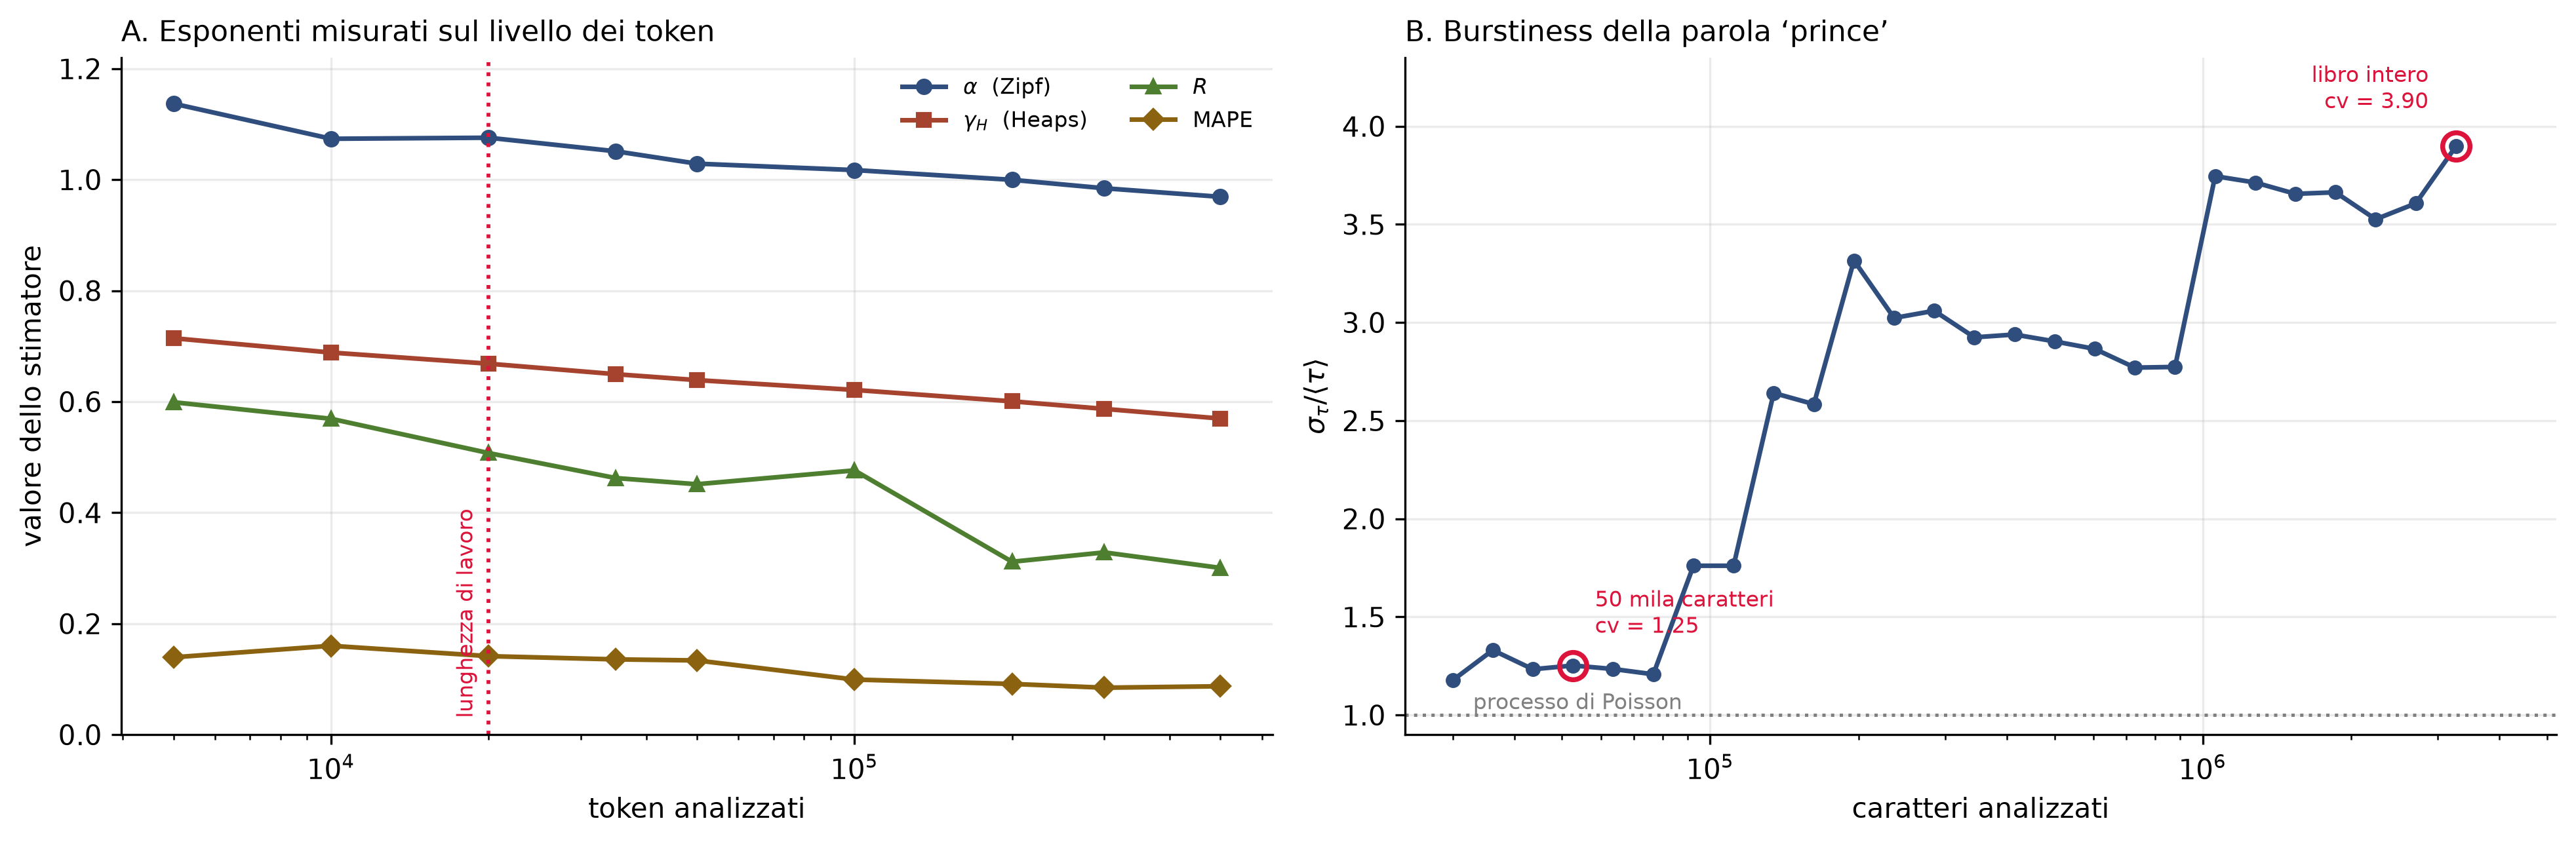
\includegraphics[width=\textwidth]{figure/cap3_dimensione_finita.png}
  \caption{Deriva degli stimatori con la lunghezza di analisi, misurata sulla
  continuazione di \emph{Guerra e pace} usata come baseline umana.
  \textbf{A}: gli esponenti misurati sul livello dei token decrescono tutti in
  modo monotono. Fra \num{5000} e \num{500000} token il descrittore $R$ passa da
  $0.60$ a $0.30$, dimezzandosi, mentre $\gamma_H$ scende da $0.72$ a $0.57$ e
  l'esponente di Zipf da $1.14$ a $0.97$. La linea verticale segna la lunghezza
  di lavoro adottata nei capitoli sperimentali.
  \textbf{B}: il coefficiente di variazione degli intervalli fra occorrenze
  della parola \emph{prince} cresce da $1.25$ su \num{50000} caratteri a $3.90$
  sul romanzo intero. La deriva è quella attesa quando la coda non
  presenta un taglio dentro la finestra osservata: finestre più lunghe
  campionano vuoti più lunghi, e la stima di $\sigma_\tau$ non raggiunge un
  valore limite. Il §\ref{sec:coda-risultati} misura direttamente il taglio e lo
  trova crescere con la finestra, da $13.5$ a $94.7$ intervalli medi fra
  \num{30000} e \num{480000} caratteri: i momenti sono finiti a ogni lunghezza,
  ma il loro valore dipende da essa.
  La Figura~\ref{fig:heaps-finito} mostrava lo stesso fenomeno su un solo
  stimatore ma su tre opere diverse, stabilendone l'universalità; qui il
  confronto è ristretto a un'unica opera e serve invece a quantificare l'entità
  dell'effetto sulla baseline effettivamente impiegata.}
  \label{fig:dimensione-finita}
\end{figure}

L'entità della deriva rende obbligatorie tre precauzioni operative, che valgono
per l'intero lavoro. Tutti i confronti fra corpora vengono condotti alla stessa
lunghezza di analisi, indicata d'ora in avanti con $N_{\mathrm{eff}}$ e
dichiarata per ciascuna fase, poiché non tutte le analisi condividono gli stessi
corpora. Nessun valore assoluto viene confrontato con valori pubblicati misurati
su lunghezze diverse. E ogni riferimento umano viene misurato con le stesse
procedure e alla stessa lunghezza dei testi con cui viene confrontato, anziché
ripreso dalla letteratura: è il paragrafo che segue. Il pannello B mostra il caso
concreto in cui la prima e la seconda precauzione si incontrano, cioè perché il
confronto con il valore pubblicato per \emph{prince} vada condotto sul romanzo
intero e non sui segmenti: è la stessa quantità, misurata su finestre che
differiscono di un fattore sessanta.

Per l'analisi appaiata dei corpora enciclopedici $N_{\mathrm{eff}}$ è fissato a
\num{60000} caratteri. Il valore è il massimo compatibile con la conservazione
di tutte le 39 terne: portandolo a \num{80000} quattro articoli non
raggiungono la soglia e le terne disponibili scendono da 39 a 35. L'intera
catena viene comunque ripetuta a quella lunghezza maggiore come controllo di
robustezza, il cui esito è riportato nel §\ref{sec:robustezza-neff} e distingue
le parti del divario che resistono al cambio di finestra da quelle che non vi
resistono.

Le altre fasi dell'analisi impiegano lunghezze diverse, perché non condividono i
corpora e non sono confrontate fra loro. La Tabella~\ref{tab:fasi} le riassume:
ciascun valore numerico che comparirà nei capitoli sperimentali è riconducibile
a una di queste righe.

\begin{table}[htbp]
\centering
\small
\begin{tabular}{@{}>{\raggedright\arraybackslash}p{2.9cm}>{\raggedright\arraybackslash}p{4.3cm}rll@{}}
\toprule
Fase & Scopo & $N_{\mathrm{eff}}$ & Unità & Analizzate \\
\midrule
Sweep di temperatura & misure sul corpus generato
  & \num{20000} & token & 242 documenti \\
\addlinespace
Raccolta & appaiamento per titolo e verifica di paternità
  & \num{80000} & caratteri & 40 coppie \\
\addlinespace
Fattibilità & verificare che l'effetto esista in prosa enciclopedica, senza
  Grokipedia & \num{50000} & caratteri & 40 voci, 20 segmenti \\
\addlinespace
Analisi principale & confronto appaiato fra i quattro corpora
  & \num{60000} & caratteri & 39 terne \\
\addlinespace
Robustezza & ripetizione dell'intera catena a lunghezza maggiore
  & \num{80000} & caratteri & 35 terne \\
\bottomrule
\end{tabular}
\caption{Le fasi dell'analisi e le rispettive lunghezze. I valori differiscono
perché le fasi non condividono i corpora, e la prima riga adotta una unità
diversa dalle altre per la ragione discussa nel §\ref{sec:unita}. Nessun
confronto attraversa righe diverse della tabella: la fase di fattibilità non
include Grokipedia, e quella sullo sweep non include alcun corpus
enciclopedico.}
\label{tab:fasi}
\end{table}

\paragraph{Baseline umana misurata, non citata.}
Per la stessa ragione, il riferimento umano non viene ripreso dalla letteratura
ma misurato con le stesse procedure e alla stessa lunghezza dei testi generati.
Il testo di riferimento è la continuazione del passaggio usato come prompt: il
confronto è quindi fra continuazione umana e continuazione generata, a parità di
contesto. La Tabella~\ref{tab:baseline} riporta i valori così ottenuti.

\begin{table}[htbp]
\centering
\small
\begin{tabular}{@{}lrr@{}}
\toprule
Grandezza & Misurata qui & Pubblicata \\
\midrule
$\alpha$ (Zipf)                 & 1.076  & $1.006 \pm 0.05$ \\
MAPE                            & 0.141  & $0.156 \pm 0.077$ \\
$\gamma_H$ (Heaps)              & 0.668  & $0.801 \pm 0.02$ \\
$R$                             & 0.507  & $0.17 \pm 0.05$ \\
$\alpha_{\mathrm{DFA}}$         & 0.579  & --- \\
$R_{\mathrm{gzip}}$             & 0.381  & --- \\
entropia [bit/carattere]        & 2.227  & --- \\
\bottomrule
\end{tabular}
\caption{Baseline umana misurata su \num{20000} token di \emph{Guerra e pace},
confrontata con i valori pubblicati in~\cite{mikhaylovskiy2025zipf}. Questi
ultimi sono calcolati su opere intere e non costituiscono un riferimento valido
per testi di questa lunghezza, per la ragione discussa nel
§\ref{sec:validazione}.}
\label{tab:baseline}
\end{table}

\paragraph{Appaiamento in frequenza dei controlli.}
Nel confronto fra parole di contenuto e parole di controllo, ciascun sostantivo
viene appaiato alla parola non-sostantivo di frequenza più vicina, minimizzando
$\lvert\log(f_w/f_k)\rvert$. L'appaiamento è indispensabile perché la burstiness
dipende dalla frequenza: confrontare parole di frequenza diversa misurerebbe
quella differenza anziché la natura semantica delle parole.

\paragraph{Selezione dei bersagli entro ciascun testo.}
Le parole bersaglio vengono scelte all'interno di ogni documento anziché fissate
una volta per tutte sul corpus di riferimento. La scelta è necessaria perché
corpora diversi trattano argomenti diversi e non condividono il lessico
tematico, ed è inoltre più efficiente, poiché produce un numero maggiore di
confronti appaiati a parità di corpus.

\paragraph{Come vengono separati i livelli lessicali.}
\label{par:livelli-lessicali}
Dentro ciascun documento le parole vengono ordinate per frequenza e ripartite in
tre insiemi. Le \emph{parole funzione} sono le sei più frequenti fra quelle che
compaiono in una lista chiusa di funtori inglesi. Le \emph{parole chiave} sono
le sette più frequenti fra quelle che superano i quattro caratteri e non
figurano in quella lista, oppure che risultano nomi propri per il criterio di
maiuscola in posizione interna alla frase descritto sopra. I \emph{controlli
appaiati} sono, per ciascuna parola chiave, la parola di frequenza più vicina
fra quelle rimaste. La ripartizione è dunque interamente determinata dalla lista
dei funtori, e la sua completezza è una scelta di metodo con conseguenze
misurabili.

La lista impiegata inizialmente conteneva \num{133} voci e ometteva alcuni
connettivi e attenuatori inglesi molto comuni, fra cui \emph{like},
\emph{amid}, \emph{including}, \emph{though}, \emph{also}, \emph{rather} e
\emph{without}. In un corpus in cui quei termini restano rari l'omissione è
innocua; in Grokipedia non lo è, perché il testo generato li impiega molto più
spesso: \emph{like} entrava fra le sette parole più frequenti in \num{29} voci
su \num{39}, contro nessuna di Wikipedia. Finivano quindi classificati come
parole chiave. Poiché i connettivi ricorrono a cadenza quasi costante e hanno
perciò burstiness bassa, il livello lessicale alto di Grokipedia risultava
contaminato da materiale che appartiene al livello dei funtori, e il divario
misurato a quel livello ne usciva gonfiato.

La lista è stata quindi estesa a \num{215} voci per classe grammaticale, cioè
preposizioni, congiunzioni subordinanti, avverbi connettivi e attenuatori e
quantificatori, e applicata identica a tutti e quattro i corpora. L'estensione
non rimuove nulla: le parole interessate passano al livello dei funtori, e al
loro posto sale fra le parole chiave la parola di contenuto successiva in
ordine di frequenza, cosicché tutti i livelli conservano la stessa numerosità
in tutti i corpora. Tutte le misure del Capitolo~\ref{cap:risultati2} sono
calcolate con la lista estesa; il §\ref{sec:effetto-stoplist} riporta di
quanto si spostano i risultati, perché lo spostamento non è trascurabile e la
scelta va resa verificabile.

% ---------------------------------------------------------------------
\section{Validazione delle procedure di calcolo}
\label{sec:validazione}

Ogni conclusione di questo lavoro poggia sul fatto che il codice misuri
effettivamente le quantità definite nel Capitolo~\ref{cap:teoria}. La
validazione procede per due vie indipendenti: la riproduzione di valori
pubblicati e la misura di grandezze il cui valore esatto è noto per costruzione.

\paragraph{Riproduzione di valori pubblicati.}
Le quantità del protocollo di Altmann sono state misurate sul corpus letterario
e confrontate con quelle riportate in~\cite{altmann2012}. Il null model A1, che
per costruzione deve restituire $\hat\gamma_{A1} \simeq 1$, dà valori compresi
fra $0.972$ e $0.984$ ai quattro livelli linguistici esaminati.

La seconda quantità riprodotta è il coefficiente di variazione della parola
\emph{prince}, che vale $3.89$ sul libro intero, in accordo con il $3.86$
pubblicato, ma scende a $1.30$ sui segmenti da \num{50000} caratteri impiegati
nei confronti. Non si tratta di un disaccordo: è la deriva di dimensione finita del
§\ref{sec:lunghezza}, e mostra perché i valori assoluti non vadano confrontati
fra lunghezze diverse. Il confronto con il valore pubblicato è quindi condotto
sul libro intero, mentre i confronti fra corpora usano la lunghezza comune.

\paragraph{Misura di esponenti noti.}
La seconda via non dipende da alcuna pubblicazione. Le procedure sono state
applicate a segnali costruiti in modo che il risultato atteso sia noto
analiticamente, ottenendo i valori della Tabella~\ref{tab:validazione}.

\begin{table}[htbp]
\centering
\small
\begin{tabular}{@{}l>{\raggedright\arraybackslash}p{5.6cm}rr@{}}
\toprule
Procedura & Segnale di prova & Atteso & Ottenuto \\
\midrule
DFA & rumore bianco & 0.500 & 0.510 \\
DFA & cammino aleatorio & 1.500 & 1.494 \\
Stimatore KL & testo confrontato con sé stesso & 0 & $0$ esatto \\
Stimatore KL & due campioni della stessa sorgente & $\simeq 0$ & 0.001 \\
Stimatore KL & sorgenti diverse & $> 0$ & 0.687 \\
\bottomrule
\end{tabular}
\caption{Validazione su segnali a esponente noto. Le prime due righe verificano
l'esponente della detrended fluctuation analysis; le ultime tre verificano che
lo stimatore della divergenza di Kullback--Leibler si annulli esattamente sul
confronto di un testo con sé stesso, resti prossimo a zero fra campioni della
stessa sorgente e cresca fra sorgenti diverse.}
\label{tab:validazione}
\end{table}

La proprietà $D(x\|x) = 0$ non è un accordo approssimato ma un'identità esatta,
e costituisce il controllo più stringente sullo stimatore della divergenza:
come discusso nel §\ref{sec:crossparsing}, essa vale soltanto se i riferimenti
usati nei due termini hanno la stessa lunghezza, e una sua violazione
segnalerebbe immediatamente l'errore.

% ---------------------------------------------------------------------
\section{Controlli di robustezza}
\label{sec:robustezza}

I controlli di questa sezione non verificano che le procedure siano corrette, ma
che i risultati non dipendano da scelte che avrebbero potuto essere compiute
diversamente.

\paragraph{Ordine del detrending.}
La detrended fluctuation analysis rimuove dalle finestre le tendenze polinomiali
fino a un grado fissato. L'intera analisi è stata condotta con il grado 1 e con
il grado 2, e la Tabella~\ref{tab:ordine-dfa} riporta le due stime a ciascuna
temperatura. Le misure riportate nel Capitolo~\ref{cap:risultati1} usano il
grado 2, per la ragione che il confronto stesso rende evidente: dove il segnale
è stazionario i due gradi coincidono, e dove non lo è il grado 1 restituisce un
esponente sistematicamente più alto, perché lascia nel segnale una tendenza che
non è correlazione.

\begin{table}[htbp]
\centering
\small
\begin{tabular}{@{}lrrrrr@{}}
\toprule
$T$ & grado 1 & grado 2 & scarto & dispersione & documenti \\
\midrule
0.4 & 0.284 & 0.307 & $-0.046$ & 0.085 & 21 \\
0.5 & 0.582 & 0.500 & $-0.132$ & 0.081 & 21 \\
0.6 & 0.613 & 0.416 & $-0.124$ & 0.093 & 21 \\
0.7 & 0.713 & 0.583 & $-0.115$ & 0.073 & 21 \\
0.8 & 0.715 & 0.601 & $-0.138$ & 0.070 & 20 \\
0.9 & 0.758 & 0.659 & $-0.078$ & 0.050 & 18 \\
1.0 & 0.753 & 0.711 & $-0.014$ & 0.054 & 17 \\
1.1 & 0.651 & 0.564 & $-0.060$ & 0.046 & 19 \\
1.2 & 0.570 & 0.556 & $-0.029$ & 0.035 & 21 \\
1.3 & 0.563 & 0.535 & $-0.007$ & 0.024 & 21 \\
1.4 & 0.535 & 0.532 & $-0.009$ & 0.019 & 21 \\
1.5 & 0.529 & 0.527 & $-0.006$ & 0.015 & 21 \\
\midrule
\multicolumn{3}{@{}l}{testo umano} & $-0.007$ & --- & 1 \\
\bottomrule
\end{tabular}
\caption{Esponente della fluttuazione stimato con detrending di grado 1 e di
grado 2. Le prime tre colonne numeriche riportano mediane sui documenti
disponibili a ciascuna temperatura; la quarta è la deviazione standard dello
scarto fra i due gradi, calcolata documento per documento. Lo scarto è negativo
ovunque, come atteso, perché il grado 2 rimuove tendenze che il grado 1 lascia
nel segnale.}
\label{tab:ordine-dfa}
\end{table}

Le due stime coincidono dove il segnale è stazionario. Sulla baseline umana lo
scarto vale $-0.007$, e sui testi generati da $T = 1.2$ in su la sua mediana vale
$-0.010$ a fronte di una dispersione fra documenti di $0.027$: la differenza fra
i due gradi è più piccola della variabilità fra documenti generati nelle stesse
condizioni, e l'esponente non dipende in modo apprezzabile dalla scelta del
detrending.

Nell'intervallo $T \in [0.5, 0.8]$ lo scarto mediano vale invece $-0.125$, con
dispersione $0.078$: qui la differenza supera nettamente la variabilità ed è
quindi reale. È concentrata nel regime in cui il testo degenera in cicli di
ripetizione e la serie dei ranghi non è stazionaria, e in quel regime,
coerentemente con quanto osservato nel §\ref{sec:ponte}, l'esponente va letto
come indicatore di periodicità e non come misura di correlazione a lungo raggio.


\paragraph{Numerosità disuguale fra celle.}
Dalla disuguale numerosità dichiarata nel §\ref{sec:protocollo} discendono due
limitazioni. Per il modello da 14 miliardi di parametri non esiste una stima
della dispersione fra campioni, cosicché nelle sue figure le barre d'errore non
sono definite e ogni suo valore è una singola realizzazione; e le deviazioni
standard riportate nelle figure del Capitolo~\ref{cap:risultati1} non sono
confrontabili fra modelli, poiché derivano da un numero diverso di campioni. Le
conclusioni che riguardano il confronto fra modelli vanno lette con questa
avvertenza, che il §\ref{sec:zipf-risultati} riprende quantitativamente sul
caso in cui pesa di più.

% ---------------------------------------------------------------------
\section{Riproducibilità}
\label{sec:riproducibilita}

Tutte le procedure sono deterministiche a semi fissati, e i semi impiegati sono
registrati nel codice. I corpora scaricati da fonti esterne sono conservati in
copia locale, così che una modifica successiva della fonte non alteri i
risultati: vale in particolare per le voci di Grokipedia, che vengono riscritte
senza cronologia pubblica.

I dati intermedi e le figure sono prodotti da notebook che salvano ogni risultato
in file separati, in formato aperto, insieme a una sintesi testuale dei
parametri usati e delle scelte compiute, così che ciascuna figura sia
ricostruibile senza ripetere i calcoli.

% =====================================================================

\chapter{Materiali e metodi}
\label{cap:metodi}

Questo capitolo descrive i corpora analizzati, il protocollo con cui i testi
artificiali sono stati prodotti e le scelte metodologiche comuni alle due parti
sperimentali. Il criterio seguito nell'esposizione è che un lettore debba poter
ripetere l'intera analisi senza dover chiedere nulla: ogni scelta viene perciò
motivata e non soltanto dichiarata.

Le ultime tre sezioni sono dedicate ai controlli. Il §\ref{sec:validazione}
verifica che le procedure di calcolo misurino effettivamente le quantità
definite nel Capitolo~\ref{cap:teoria}; il §\ref{sec:robustezza} verifica che i
risultati non dipendano da scelte arbitrarie. Sono due questioni distinte, e
tenerle separate rende più chiaro che cosa ciascun controllo dimostri.

% ---------------------------------------------------------------------
\section{I corpora}
\label{sec:corpora}

L'analisi impiega cinque corpora, riassunti nella Tabella~\ref{tab:corpora}.
Due sono di riferimento umano, due sono enciclopedie messe a confronto fra loro,
e uno raccoglie i testi generati automaticamente.

\begin{table}[htbp]
\centering
\small
\begin{tabular}{@{}l>{\raggedright\arraybackslash}p{5.9cm}c@{}}
\toprule
Corpus & Provenienza e criterio di selezione & Unità \\
\midrule
\emph{Guerra e pace} & Project Gutenberg; segmenti contigui di uguale lunghezza,
usati come ancora al protocollo originale & 20 segmenti \\
\addlinespace
Wikipedia & voci a tema ampio, selezionate ordinando per lunghezza di prosa
effettiva & 40 raccolte, 39 analizzate \\
\addlinespace
Grokipedia (attuale) & le stesse voci, appaiate per titolo & 40 raccolte, 39
analizzate \\
\addlinespace
Grokipedia v0.1 & le stesse voci nella versione di ottobre 2025, recuperata da
Internet Archive & 40 raccolte, 39 analizzate \\
\addlinespace
Testi generati & cinque modelli Qwen, sweep di temperatura descritto nel
§\ref{sec:protocollo} & 242 documenti \\
\bottomrule
\end{tabular}
\caption{I corpora analizzati.}
\label{tab:corpora}
\end{table}

Il corpus letterario ha una funzione precisa: fornire un'ancora al protocollo di
Altmann~\cite{altmann2012}, che è stato formulato e validato su romanzi. I valori
misurati su di esso permettono di verificare che la procedura riproduca quanto
pubblicato prima di applicarla a testi di natura diversa.

Le voci di Wikipedia sono state ordinate per lunghezza del solo testo corrente,
dopo rimozione di marcatura, tabelle, note e riferimenti. I due criteri più
immediati non sono utilizzabili. Ordinare le pagine per dimensione del sorgente
wiki restituisce liste, tabelle e infobox anziché prosa: una pagina da
\num{679016} byte di sorgente conteneva \num{1284} caratteri di prosa effettiva.
Ordinare per qualità editoriale è ugualmente inadatto, poiché le voci in vetrina
sono selezionate per accuratezza e non per lunghezza.

Grokipedia compare in due versioni perché la piattaforma non pubblica una
cronologia delle revisioni. La versione di ottobre 2025 è stata recuperata da
Internet Archive, disponibile per tutte e quaranta le voci, e consente di
verificare se gli indicatori misurati cambino a seguito della revisione
editoriale: è il controllo riportato nel Capitolo~\ref{cap:risultati2}.

% ---------------------------------------------------------------------
\section{Protocollo di generazione}
\label{sec:protocollo}

I testi artificiali sono stati prodotti da cinque modelli della famiglia Qwen,
elencati nella Tabella~\ref{tab:modelli}. Tutti sono modelli \emph{base}, cioè
non sottoposti ad affinamento su istruzioni: la scelta isola le proprietà del
modello linguistico da quelle indotte dall'addestramento successivo, che
in~\cite{mikhaylovskiy2025zipf} risultano spostare sensibilmente il
comportamento statistico.

\begin{table}[htbp]
\centering
\small
\begin{tabular}{@{}llrlr@{}}
\toprule
Modello & Famiglia & Parametri & Architettura & Documenti \\
\midrule
Qwen2.5-1.5B     & Qwen2.5 & 1.54\,G  & transformer denso & 57 \\
Qwen2.5-3B       & Qwen2.5 & 3.09\,G  & transformer denso & 53 \\
Qwen2.5-14B      & Qwen2.5 & 14.7\,G  & transformer denso & 12 \\
Qwen3.5-2B-Base  & Qwen3.5 & 2.0\,G   & ibrida            & 60 \\
Qwen3.5-4B-Base  & Qwen3.5 & 4.0\,G   & ibrida            & 60 \\
\midrule
\multicolumn{4}{@{}l}{totale} & 242 \\
\bottomrule
\end{tabular}
\caption{I cinque modelli impiegati. L'intervallo di dimensioni copre un ordine
di grandezza, e le due famiglie differiscono per architettura. I modelli
Qwen2.5 sono transformer densi ad attenzione completa su tutti gli strati; i
modelli Qwen3.5 sono ibridi e ripetono un blocco di quattro strati in cui tre
impiegano attenzione lineare e uno attenzione completa. Le schede ufficiali
riportano \num{24} strati per il modello da 2 miliardi di parametri, come
$6\times(3\times\text{lineare} + 1\times\text{completa})$, e \num{32} per
quello da 4 miliardi, come $8\times(3+1)$: in entrambi i casi tre quarti degli
strati sono ad attenzione lineare.}
\label{tab:modelli}
\end{table}

Ogni modello ha generato testo a dodici temperature, da $T = 0.4$ a $T = 1.5$
con passo $0.1$. Il prompt è identico per tutti: un blocco di 2000 token tratto
da \emph{Guerra e pace}, la cui posizione esatta nel romanzo è stata verificata
come descritto nel §\ref{sec:paternita}. Ciascuna generazione produce
\num{24000} token di completamento, misurati con il tokenizzatore del modello
generante.

\paragraph{Che cosa comporta un prompt lungo.}
La scelta di un prompt di 2000 token non è neutra rispetto alle misure, e la
conseguenza è anticipata qui perché ricorre in tutto il
Capitolo~\ref{cap:risultati1}. La sezione 4.5
di~\cite{mikhaylovskiy2025zipf} ripete lo sweep con un prompt di quella
lunghezza tratto da un testo naturale e osserva che la ricchezza lessicale del
prompt domina il vocabolario, relativamente piccolo, del testo generato: alcuni
modelli non producono alcun tipo nuovo alle basse temperature, i massimi delle
curve del descrittore $R$ si spostano verso le temperature alte, e l'errore del
fit di Zipf si abbassa soprattutto nella regione a bassa temperatura. Le
proprietà del regime disordinato compaiono dunque più tardi, e quelle del
regime ordinato persistono più a lungo, di quanto si osserverebbe generando da
un singolo token. I confronti con i valori pubblicati vanno letti tenendone
conto, e i punti in cui l'effetto si manifesta sono segnalati di volta in
volta.

Il campionamento impiega la sola temperatura. I parametri che troncano la
distribuzione sono disattivati, con $\mathrm{top}\text{-}p = 1$ e
$\mathrm{top}\text{-}k = -1$, e la penalità di ripetizione è posta a 1. È la
condizione richiesta dal §\ref{sec:temperatura}: qualunque altro parametro
introdurrebbe un secondo grado di libertà e renderebbe impossibile attribuire
alla sola temperatura il comportamento osservato.

\paragraph{Generazione in continuazione.}
Per raggiungere i \num{24000} token richiesti la generazione riparte dopo ogni
token di fine sequenza, riprendendo dal testo accumulato fino a quel punto. I
documenti prodotti sono dunque ricuciti da più segmenti, in numero variabile fino
a un massimo di 27 riprese per campione. Poiché un modello autoregressivo è privo
di stato interno persistente, riprendere dal testo accumulato produce la stessa
distribuzione condizionata. Un confronto a temperatura fissata fra i documenti
ricuciti da più segmenti e quelli generati in un colpo solo non rivela
differenze nelle due misure sensibili all'ordine, entro la dispersione dei dati;
il confronto ha però poca potenza, perché sotto $T = 0.9$ i documenti con
riprese sono pochissimi e sopra $T = 1.0$ la ripetizione è già nulla.

\paragraph{Numerosità disuguale.}
Il numero di documenti per modello non è uniforme, e la
Tabella~\ref{tab:modelli} lo riporta esplicitamente: il modello da 14 miliardi
di parametri dispone di un solo campione per temperatura, contro i cinque della
maggior parte degli altri. Le conseguenze sono discusse fra i limiti nel
§\ref{sec:robustezza}.

% ---------------------------------------------------------------------
\section{Verifica di paternità dei corpora}
\label{sec:paternita}

Il confronto fra Wikipedia e Grokipedia presuppone che le voci della seconda
siano effettivamente scritte da un modello generativo e non ricopiate dalla
prima. La verifica misura la sovrapposizione di 8-grammi fra le due versioni di
ciascuna voce: sul corpus attuale la mediana vale $0.0003$ e il massimo $0.046$,
valori che escludono la derivazione testuale diretta. Una voce della versione
v0.1, \emph{Buddhism}, risultava invece ricopiata all'84\% ed è stata esclusa
dall'analisi appaiata, che si riduce quindi a 39 terne: il disegno richiede
infatti che tutte e tre le versioni siano disponibili per ogni titolo, per cui
l'esclusione di una versione comporta quella dell'intera terna.

Per i testi generati la verifica riguarda il prompt. Poiché i cinque dataset sono
stati prodotti in momenti diversi, occorre accertare che partano tutti dallo
stesso punto del romanzo. Il controllo non è stato condotto per ispezione ma per
funzione di hash: dell'impronta SHA-256 registrata in ciascun dataset è stata
cercata la corrispondenza nel testo del romanzo, individuando l'offset esatto in
caratteri. Tutti e cinque i dataset risultano partire dalla stessa posizione. Due
di essi registrano una lunghezza del prompt di poco diversa, \num{8239} contro
\num{8262} caratteri, differenza dovuta al punto in cui cade il confine dei 2000
token con i due tokenizzatori delle rispettive famiglie e non a un testo diverso.

% ---------------------------------------------------------------------
\section{Unità di analisi}
\label{sec:unita}

La scelta dell'unità in cui misurare i testi è la decisione metodologica di
maggiore conseguenza dell'intero lavoro, e viene qui motivata per esteso.

Il livello primario è il token, non la parola. La ragione, già anticipata nel
§\ref{sec:token}, è che alle temperature alte i modelli producono sequenze non
interpretabili come parole: una tokenizzazione lessicale misurerebbe in quel
regime artefatti della segmentazione anziché proprietà del testo. La stessa
scelta, e per lo stesso motivo, è compiuta in~\cite{mikhaylovskiy2025zipf}.

Il tokenizzatore impiegato nell'analisi è unico per tutti i corpora ed è esterno
alle famiglie che hanno generato i testi. Le due condizioni sono entrambe
necessarie. L'unicità serve a rendere confrontabili gli esponenti misurati su
modelli diversi: i tokenizzatori di Qwen2.5 e Qwen3.5 segmentano lo stesso testo
in modo diverso, e misurare ciascun modello con il proprio metro produrrebbe
differenze attribuibili alla segmentazione anziché al testo. L'esternalità serve
a evitare che un modello risulti favorito dal fatto di essere misurato con il
proprio vocabolario. La scelta ricalca quella di~\cite{mikhaylovskiy2025zipf},
dove testi prodotti da quattro famiglie distinte vengono analizzati con un
tokenizzatore che non appartiene a nessuna di esse.

In concreto l'analisi impiega \texttt{cl100k\_base}, con \num{100277} voci.
Cambiare tokenizzatore sposta i valori assoluti degli esponenti, poiché cambia
l'unità in cui si contano le occorrenze, ma non la posizione dei loro estremi in
funzione della temperatura, che è la quantità su cui poggiano le conclusioni del
Capitolo~\ref{cap:risultati1}.

Ogni documento generato viene troncato ai primi \num{20000} token di analisi, e
la baseline umana è misurata sulla stessa quantità. Il valore è il massimo
compatibile con il documento più corto del corpus: la generazione produce
\num{24000} token misurati con il tokenizzatore del modello generante, che
\texttt{cl100k\_base} risegmenta in un numero variabile di token di analisi, e
troncare a una soglia comune è indispensabile perché tutte le misure del
Capitolo~\ref{cap:risultati1} dipendono dalla lunghezza. La prima riga della
Tabella~\ref{tab:fasi} riporta questa fase; le altre adottano il carattere come
unità, perché il protocollo del §\ref{sec:burst} misura le distanze in
caratteri.

Il livello lessicale resta impiegato, in funzione secondaria, per le misure che
sono definite sulle parole: la diversità lessicale, le distanze di ripetizione,
gli $n$-grammi ripetuti e la mappatura sui vettori di embedding. La detrended
fluctuation analysis fa eccezione a entrambi i livelli, poiché
in~\cite{lippi2019} è definita sui caratteri, e qui si segue quella definizione.

% ---------------------------------------------------------------------
\section{Scelte metodologiche trasversali}
\label{sec:scelte}

Quattro decisioni attraversano entrambe le parti sperimentali.

\paragraph{Lunghezza di analisi comune.}
Come anticipato nel §\ref{sec:lunghezza}, diversi stimatori impiegati in questo
lavoro non convergono al crescere della lunghezza del testo, ma derivano in modo
sistematico. La Figura~\ref{fig:dimensione-finita} misura la deriva su un testo
umano, e mostra che non si tratta di un effetto trascurabile.

\begin{figure}[htbp]
  \centering
  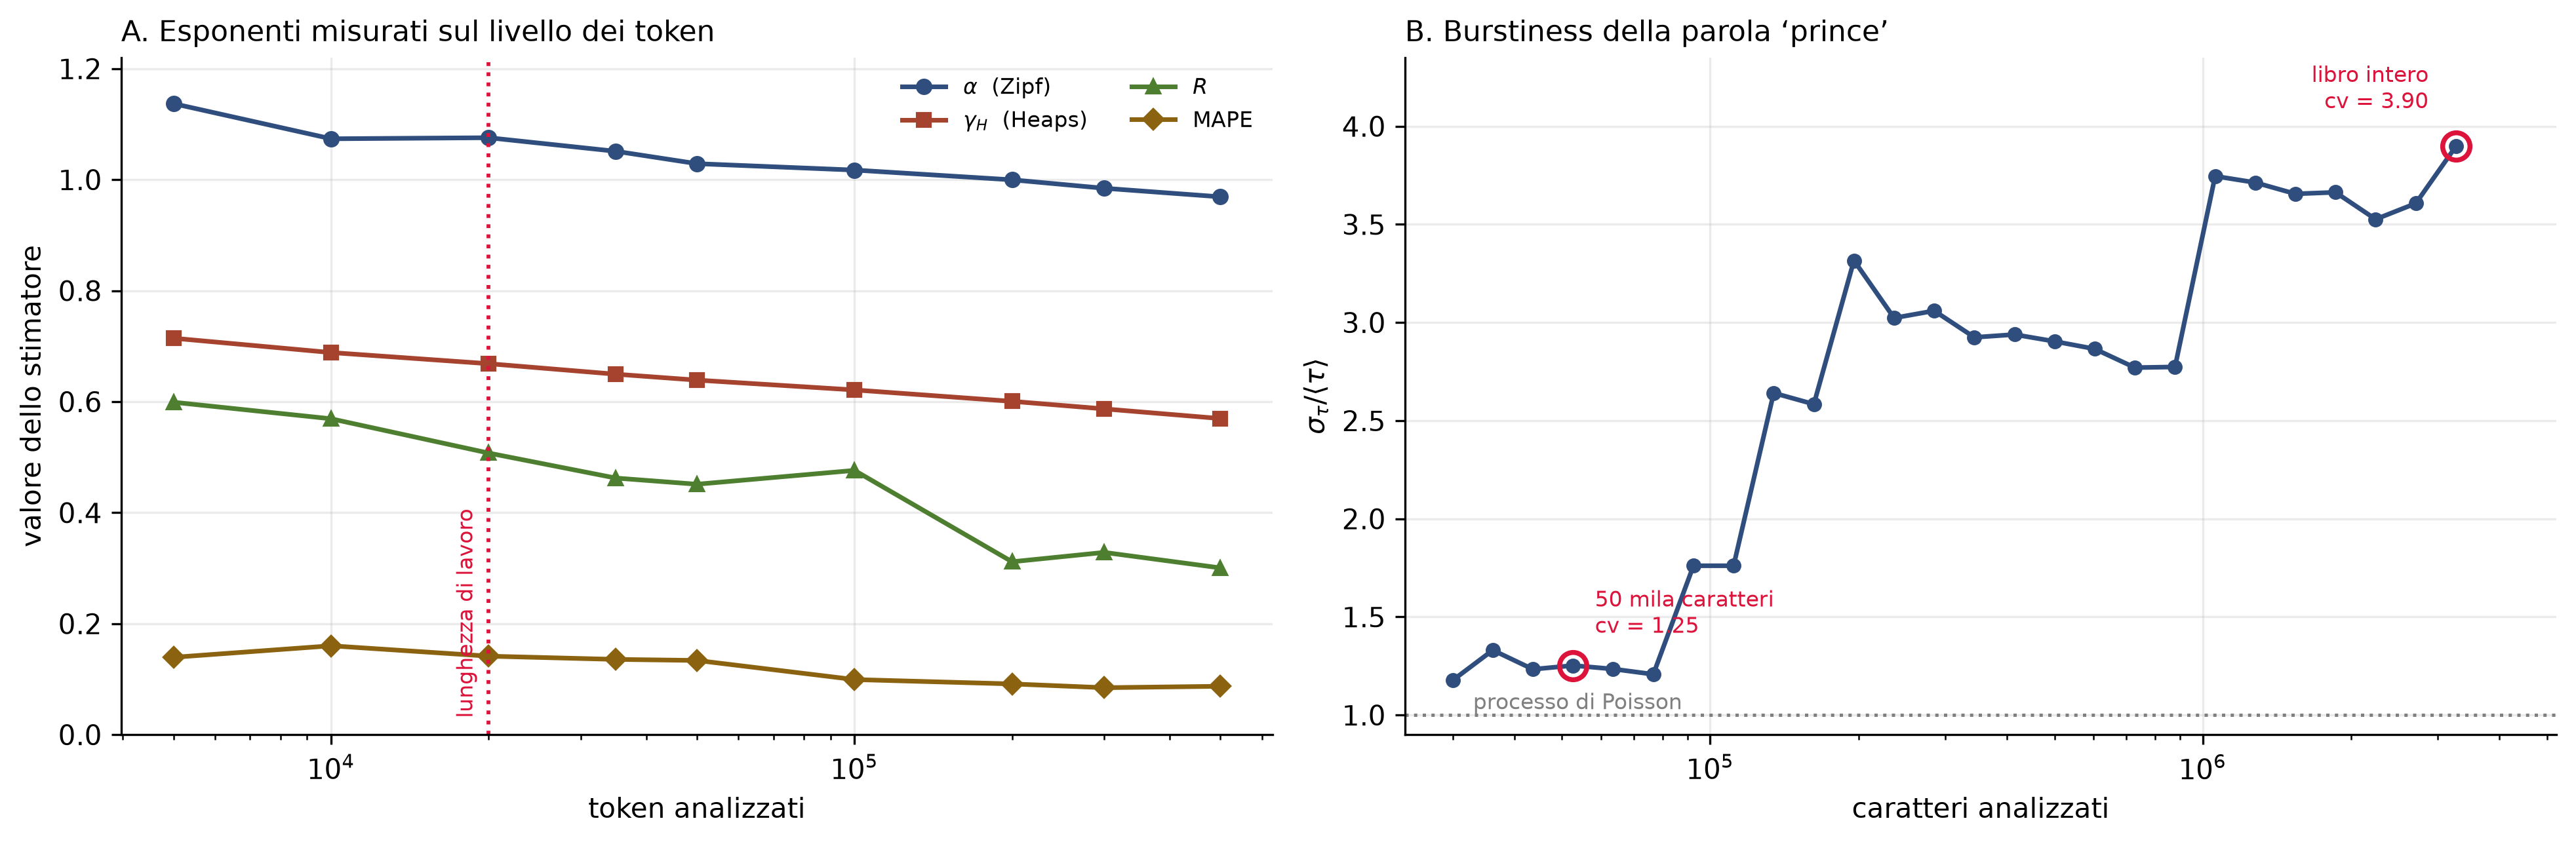
\includegraphics[width=\textwidth]{figure/cap3_dimensione_finita.png}
  \caption{Deriva degli stimatori con la lunghezza di analisi, misurata sulla
  continuazione di \emph{Guerra e pace} usata come baseline umana.
  \textbf{A}: gli esponenti misurati sul livello dei token decrescono tutti in
  modo monotono. Fra \num{5000} e \num{500000} token il descrittore $R$ passa da
  $0.60$ a $0.30$, dimezzandosi, mentre $\gamma_H$ scende da $0.72$ a $0.57$ e
  l'esponente di Zipf da $1.14$ a $0.97$. La linea verticale segna la lunghezza
  di lavoro adottata nei capitoli sperimentali.
  \textbf{B}: il coefficiente di variazione degli intervalli fra occorrenze
  della parola \emph{prince} cresce da $1.25$ su \num{50000} caratteri a $3.90$
  sul romanzo intero. La deriva è quella attesa quando la coda non
  presenta un taglio dentro la finestra osservata: finestre più lunghe
  campionano vuoti più lunghi, e la stima di $\sigma_\tau$ non raggiunge un
  valore limite. Il §\ref{sec:coda-risultati} misura direttamente il taglio e lo
  trova crescere con la finestra, da $13.5$ a $94.7$ intervalli medi fra
  \num{30000} e \num{480000} caratteri: i momenti sono finiti a ogni lunghezza,
  ma il loro valore dipende da essa.
  La Figura~\ref{fig:heaps-finito} mostrava lo stesso fenomeno su un solo
  stimatore ma su tre opere diverse, stabilendone l'universalità; qui il
  confronto è ristretto a un'unica opera e serve invece a quantificare l'entità
  dell'effetto sulla baseline effettivamente impiegata.}
  \label{fig:dimensione-finita}
\end{figure}

L'entità della deriva rende obbligatorie tre precauzioni operative, che valgono
per l'intero lavoro. Tutti i confronti fra corpora vengono condotti alla stessa
lunghezza di analisi, indicata d'ora in avanti con $N_{\mathrm{eff}}$ e
dichiarata per ciascuna fase, poiché non tutte le analisi condividono gli stessi
corpora. Nessun valore assoluto viene confrontato con valori pubblicati misurati
su lunghezze diverse. E ogni riferimento umano viene misurato con le stesse
procedure e alla stessa lunghezza dei testi con cui viene confrontato, anziché
ripreso dalla letteratura: è il paragrafo che segue. Il pannello B mostra il caso
concreto in cui la prima e la seconda precauzione si incontrano, cioè perché il
confronto con il valore pubblicato per \emph{prince} vada condotto sul romanzo
intero e non sui segmenti: è la stessa quantità, misurata su finestre che
differiscono di un fattore sessanta.

Per l'analisi appaiata dei corpora enciclopedici $N_{\mathrm{eff}}$ è fissato a
\num{60000} caratteri. Il valore è il massimo compatibile con la conservazione
di tutte le 39 terne: portandolo a \num{80000} quattro articoli non
raggiungono la soglia e le terne disponibili scendono da 39 a 35. L'intera
catena viene comunque ripetuta a quella lunghezza maggiore come controllo di
robustezza, il cui esito è riportato nel §\ref{sec:robustezza-neff} e distingue
le parti del divario che resistono al cambio di finestra da quelle che non vi
resistono.

Le altre fasi dell'analisi impiegano lunghezze diverse, perché non condividono i
corpora e non sono confrontate fra loro. La Tabella~\ref{tab:fasi} le riassume:
ciascun valore numerico che comparirà nei capitoli sperimentali è riconducibile
a una di queste righe.

\begin{table}[htbp]
\centering
\small
\begin{tabular}{@{}>{\raggedright\arraybackslash}p{2.9cm}>{\raggedright\arraybackslash}p{4.3cm}rll@{}}
\toprule
Fase & Scopo & $N_{\mathrm{eff}}$ & Unità & Analizzate \\
\midrule
Sweep di temperatura & misure sul corpus generato
  & \num{20000} & token & 242 documenti \\
\addlinespace
Raccolta & appaiamento per titolo e verifica di paternità
  & \num{80000} & caratteri & 40 coppie \\
\addlinespace
Fattibilità & verificare che l'effetto esista in prosa enciclopedica, senza
  Grokipedia & \num{50000} & caratteri & 40 voci, 20 segmenti \\
\addlinespace
Analisi principale & confronto appaiato fra i quattro corpora
  & \num{60000} & caratteri & 39 terne \\
\addlinespace
Robustezza & ripetizione dell'intera catena a lunghezza maggiore
  & \num{80000} & caratteri & 35 terne \\
\bottomrule
\end{tabular}
\caption{Le fasi dell'analisi e le rispettive lunghezze. I valori differiscono
perché le fasi non condividono i corpora, e la prima riga adotta una unità
diversa dalle altre per la ragione discussa nel §\ref{sec:unita}. Nessun
confronto attraversa righe diverse della tabella: la fase di fattibilità non
include Grokipedia, e quella sullo sweep non include alcun corpus
enciclopedico.}
\label{tab:fasi}
\end{table}

\paragraph{Baseline umana misurata, non citata.}
Per la stessa ragione, il riferimento umano non viene ripreso dalla letteratura
ma misurato con le stesse procedure e alla stessa lunghezza dei testi generati.
Il testo di riferimento è la continuazione del passaggio usato come prompt: il
confronto è quindi fra continuazione umana e continuazione generata, a parità di
contesto. La Tabella~\ref{tab:baseline} riporta i valori così ottenuti.

\begin{table}[htbp]
\centering
\small
\begin{tabular}{@{}lrr@{}}
\toprule
Grandezza & Misurata qui & Pubblicata \\
\midrule
$\alpha$ (Zipf)                 & 1.076  & $1.006 \pm 0.05$ \\
MAPE                            & 0.141  & $0.156 \pm 0.077$ \\
$\gamma_H$ (Heaps)              & 0.668  & $0.801 \pm 0.02$ \\
$R$                             & 0.507  & $0.17 \pm 0.05$ \\
$\alpha_{\mathrm{DFA}}$         & 0.579  & --- \\
$R_{\mathrm{gzip}}$             & 0.381  & --- \\
entropia [bit/carattere]        & 2.227  & --- \\
\bottomrule
\end{tabular}
\caption{Baseline umana misurata su \num{20000} token di \emph{Guerra e pace},
confrontata con i valori pubblicati in~\cite{mikhaylovskiy2025zipf}. Questi
ultimi sono calcolati su opere intere e non costituiscono un riferimento valido
per testi di questa lunghezza, per la ragione discussa nel
§\ref{sec:validazione}.}
\label{tab:baseline}
\end{table}

\paragraph{Appaiamento in frequenza dei controlli.}
Nel confronto fra parole di contenuto e parole di controllo, ciascun sostantivo
viene appaiato alla parola non-sostantivo di frequenza più vicina, minimizzando
$\lvert\log(f_w/f_k)\rvert$. L'appaiamento è indispensabile perché la burstiness
dipende dalla frequenza: confrontare parole di frequenza diversa misurerebbe
quella differenza anziché la natura semantica delle parole.

\paragraph{Selezione dei bersagli entro ciascun testo.}
Le parole bersaglio vengono scelte all'interno di ogni documento anziché fissate
una volta per tutte sul corpus di riferimento. La scelta è necessaria perché
corpora diversi trattano argomenti diversi e non condividono il lessico
tematico, ed è inoltre più efficiente, poiché produce un numero maggiore di
confronti appaiati a parità di corpus.

\paragraph{Come vengono separati i livelli lessicali.}
\label{par:livelli-lessicali}
Dentro ciascun documento le parole vengono ordinate per frequenza e ripartite in
tre insiemi. Le \emph{parole funzione} sono le sei più frequenti fra quelle che
compaiono in una lista chiusa di funtori inglesi. Le \emph{parole chiave} sono
le sette più frequenti fra quelle che superano i quattro caratteri e non
figurano in quella lista, oppure che risultano nomi propri per il criterio di
maiuscola in posizione interna alla frase descritto sopra. I \emph{controlli
appaiati} sono, per ciascuna parola chiave, la parola di frequenza più vicina
fra quelle rimaste. La ripartizione è dunque interamente determinata dalla lista
dei funtori, e la sua completezza è una scelta di metodo con conseguenze
misurabili.

La lista impiegata inizialmente conteneva \num{133} voci e ometteva alcuni
connettivi e attenuatori inglesi molto comuni, fra cui \emph{like},
\emph{amid}, \emph{including}, \emph{though}, \emph{also}, \emph{rather} e
\emph{without}. In un corpus in cui quei termini restano rari l'omissione è
innocua; in Grokipedia non lo è, perché il testo generato li impiega molto più
spesso: \emph{like} entrava fra le sette parole più frequenti in \num{29} voci
su \num{39}, contro nessuna di Wikipedia. Finivano quindi classificati come
parole chiave. Poiché i connettivi ricorrono a cadenza quasi costante e hanno
perciò burstiness bassa, il livello lessicale alto di Grokipedia risultava
contaminato da materiale che appartiene al livello dei funtori, e il divario
misurato a quel livello ne usciva gonfiato.

La lista è stata quindi estesa a \num{215} voci per classe grammaticale, cioè
preposizioni, congiunzioni subordinanti, avverbi connettivi e attenuatori e
quantificatori, e applicata identica a tutti e quattro i corpora. L'estensione
non rimuove nulla: le parole interessate passano al livello dei funtori, e al
loro posto sale fra le parole chiave la parola di contenuto successiva in
ordine di frequenza, cosicché tutti i livelli conservano la stessa numerosità
in tutti i corpora. Tutte le misure del Capitolo~\ref{cap:risultati2} sono
calcolate con la lista estesa; il §\ref{sec:effetto-stoplist} riporta di
quanto si spostano i risultati, perché lo spostamento non è trascurabile e la
scelta va resa verificabile.

% ---------------------------------------------------------------------
\section{Validazione delle procedure di calcolo}
\label{sec:validazione}

Ogni conclusione di questo lavoro poggia sul fatto che il codice misuri
effettivamente le quantità definite nel Capitolo~\ref{cap:teoria}. La
validazione procede per due vie indipendenti: la riproduzione di valori
pubblicati e la misura di grandezze il cui valore esatto è noto per costruzione.

\paragraph{Riproduzione di valori pubblicati.}
Le quantità del protocollo di Altmann sono state misurate sul corpus letterario
e confrontate con quelle riportate in~\cite{altmann2012}. Il null model A1, che
per costruzione deve restituire $\hat\gamma_{A1} \simeq 1$, dà valori compresi
fra $0.972$ e $0.984$ ai quattro livelli linguistici esaminati.

La seconda quantità riprodotta è il coefficiente di variazione della parola
\emph{prince}, che vale $3.89$ sul libro intero, in accordo con il $3.86$
pubblicato, ma scende a $1.30$ sui segmenti da \num{50000} caratteri impiegati
nei confronti. Non si tratta di un disaccordo: è la deriva di dimensione finita del
§\ref{sec:lunghezza}, e mostra perché i valori assoluti non vadano confrontati
fra lunghezze diverse. Il confronto con il valore pubblicato è quindi condotto
sul libro intero, mentre i confronti fra corpora usano la lunghezza comune.

\paragraph{Misura di esponenti noti.}
La seconda via non dipende da alcuna pubblicazione. Le procedure sono state
applicate a segnali costruiti in modo che il risultato atteso sia noto
analiticamente, ottenendo i valori della Tabella~\ref{tab:validazione}.

\begin{table}[htbp]
\centering
\small
\begin{tabular}{@{}l>{\raggedright\arraybackslash}p{5.6cm}rr@{}}
\toprule
Procedura & Segnale di prova & Atteso & Ottenuto \\
\midrule
DFA & rumore bianco & 0.500 & 0.510 \\
DFA & cammino aleatorio & 1.500 & 1.494 \\
Stimatore KL & testo confrontato con sé stesso & 0 & $0$ esatto \\
Stimatore KL & due campioni della stessa sorgente & $\simeq 0$ & 0.001 \\
Stimatore KL & sorgenti diverse & $> 0$ & 0.687 \\
\bottomrule
\end{tabular}
\caption{Validazione su segnali a esponente noto. Le prime due righe verificano
l'esponente della detrended fluctuation analysis; le ultime tre verificano che
lo stimatore della divergenza di Kullback--Leibler si annulli esattamente sul
confronto di un testo con sé stesso, resti prossimo a zero fra campioni della
stessa sorgente e cresca fra sorgenti diverse.}
\label{tab:validazione}
\end{table}

La proprietà $D(x\|x) = 0$ non è un accordo approssimato ma un'identità esatta,
e costituisce il controllo più stringente sullo stimatore della divergenza:
come discusso nel §\ref{sec:crossparsing}, essa vale soltanto se i riferimenti
usati nei due termini hanno la stessa lunghezza, e una sua violazione
segnalerebbe immediatamente l'errore.

% ---------------------------------------------------------------------
\section{Controlli di robustezza}
\label{sec:robustezza}

I controlli di questa sezione non verificano che le procedure siano corrette, ma
che i risultati non dipendano da scelte che avrebbero potuto essere compiute
diversamente.

\paragraph{Ordine del detrending.}
La detrended fluctuation analysis rimuove dalle finestre le tendenze polinomiali
fino a un grado fissato. L'intera analisi è stata condotta con il grado 1 e con
il grado 2, e la Tabella~\ref{tab:ordine-dfa} riporta le due stime a ciascuna
temperatura. Le misure riportate nel Capitolo~\ref{cap:risultati1} usano il
grado 2, per la ragione che il confronto stesso rende evidente: dove il segnale
è stazionario i due gradi coincidono, e dove non lo è il grado 1 restituisce un
esponente sistematicamente più alto, perché lascia nel segnale una tendenza che
non è correlazione.

\begin{table}[htbp]
\centering
\small
\begin{tabular}{@{}lrrrrr@{}}
\toprule
$T$ & grado 1 & grado 2 & scarto & dispersione & documenti \\
\midrule
0.4 & 0.284 & 0.307 & $-0.046$ & 0.085 & 21 \\
0.5 & 0.582 & 0.500 & $-0.132$ & 0.081 & 21 \\
0.6 & 0.613 & 0.416 & $-0.124$ & 0.093 & 21 \\
0.7 & 0.713 & 0.583 & $-0.115$ & 0.073 & 21 \\
0.8 & 0.715 & 0.601 & $-0.138$ & 0.070 & 20 \\
0.9 & 0.758 & 0.659 & $-0.078$ & 0.050 & 18 \\
1.0 & 0.753 & 0.711 & $-0.014$ & 0.054 & 17 \\
1.1 & 0.651 & 0.564 & $-0.060$ & 0.046 & 19 \\
1.2 & 0.570 & 0.556 & $-0.029$ & 0.035 & 21 \\
1.3 & 0.563 & 0.535 & $-0.007$ & 0.024 & 21 \\
1.4 & 0.535 & 0.532 & $-0.009$ & 0.019 & 21 \\
1.5 & 0.529 & 0.527 & $-0.006$ & 0.015 & 21 \\
\midrule
\multicolumn{3}{@{}l}{testo umano} & $-0.007$ & --- & 1 \\
\bottomrule
\end{tabular}
\caption{Esponente della fluttuazione stimato con detrending di grado 1 e di
grado 2. Le prime tre colonne numeriche riportano mediane sui documenti
disponibili a ciascuna temperatura; la quarta è la deviazione standard dello
scarto fra i due gradi, calcolata documento per documento. Lo scarto è negativo
ovunque, come atteso, perché il grado 2 rimuove tendenze che il grado 1 lascia
nel segnale.}
\label{tab:ordine-dfa}
\end{table}

Le due stime coincidono dove il segnale è stazionario. Sulla baseline umana lo
scarto vale $-0.007$, e sui testi generati da $T = 1.2$ in su la sua mediana vale
$-0.010$ a fronte di una dispersione fra documenti di $0.027$: la differenza fra
i due gradi è più piccola della variabilità fra documenti generati nelle stesse
condizioni, e l'esponente non dipende in modo apprezzabile dalla scelta del
detrending.

Nell'intervallo $T \in [0.5, 0.8]$ lo scarto mediano vale invece $-0.125$, con
dispersione $0.078$: qui la differenza supera nettamente la variabilità ed è
quindi reale. È concentrata nel regime in cui il testo degenera in cicli di
ripetizione e la serie dei ranghi non è stazionaria, e in quel regime,
coerentemente con quanto osservato nel §\ref{sec:ponte}, l'esponente va letto
come indicatore di periodicità e non come misura di correlazione a lungo raggio.


\paragraph{Numerosità disuguale fra celle.}
Dalla disuguale numerosità dichiarata nel §\ref{sec:protocollo} discendono due
limitazioni. Per il modello da 14 miliardi di parametri non esiste una stima
della dispersione fra campioni, cosicché nelle sue figure le barre d'errore non
sono definite e ogni suo valore è una singola realizzazione; e le deviazioni
standard riportate nelle figure del Capitolo~\ref{cap:risultati1} non sono
confrontabili fra modelli, poiché derivano da un numero diverso di campioni. Le
conclusioni che riguardano il confronto fra modelli vanno lette con questa
avvertenza, che il §\ref{sec:zipf-risultati} riprende quantitativamente sul
caso in cui pesa di più.

% ---------------------------------------------------------------------
\section{Riproducibilità}
\label{sec:riproducibilita}

Tutte le procedure sono deterministiche a semi fissati, e i semi impiegati sono
registrati nel codice. I corpora scaricati da fonti esterne sono conservati in
copia locale, così che una modifica successiva della fonte non alteri i
risultati: vale in particolare per le voci di Grokipedia, che vengono riscritte
senza cronologia pubblica.

I dati intermedi e le figure sono prodotti da notebook che salvano ogni risultato
in file separati, in formato aperto, insieme a una sintesi testuale dei
parametri usati e delle scelte compiute, così che ciascuna figura sia
ricostruibile senza ripetere i calcoli.
